\chapter{Results} \label{chap:results}

\bigskip
\section{The Unexpected Results}

In the first stage of the experiment, after comparing the two frameworks running sorting algorithms, we discovered that Flask has a better performance than Spin in contrast to our initial hypothesis. Therefore, we decided to expand on the algorithm comparison and further introduce 4 more minimum distance and spanning tree algorithms. They are Dijkstra' Algorithm, Floyd's Algorithm, Kruskal's Algorithm and Prim's Algorithm.

As shown in the figure below, in both stages of the experiment, the Flask framework consistently outpaced the WebAssembly Spin framework with some algorithms benchmarking more than 100\% faster. In this section, we will dive deeper into the data and analyse the reason behind such inconsistent behaviour.

In the first stage of the experiment, we compared the runtime performance across 3 platforms: native in the local environment, online production via Flask and online production via Spin. The native environment is marked with the blue bar, Flask with orange and Spin with grey. Comparing the runtime performance between Flask and Spin, we clearly notice a visible performance gap. Across \textbf{18} benchmarking algorithms running \textbf{54} tests in total, only \textbf{1} algorithm across \textbf{3} tests, or \textbf{5.6} percent of the times where Spin outperformed Flask \textbf{(Bucket Sort)}. In this case, the runtime for Spin is \textbf{2.28s, 6.07s, 10.5s} for small, medium and large input sizes, respectively. This was faster than Flask's runtime, which was \textbf{2.38s, 6.82s and 11.95s} on average across running the algorithm \textbf{5} times.

Here is the runtime comparison across all 18 benchmarking algorithms (average of 5 runs):

\newpage
\bigskip
\begin{figure}[hp]
\centering
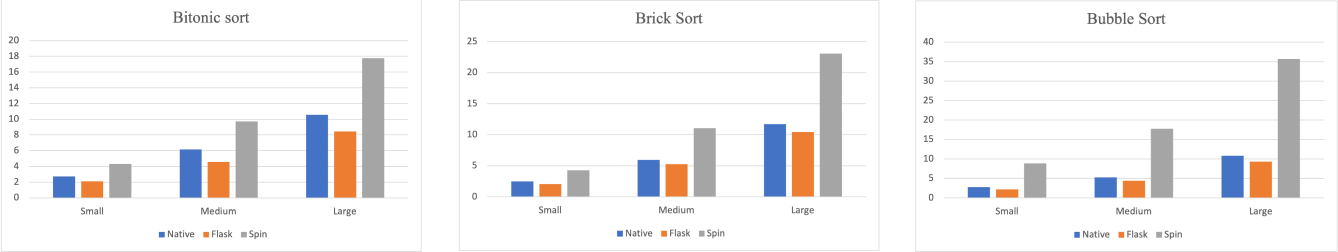
\includegraphics[scale=0.33]{sort1}
\caption{\footnotesize{Benchmark on Bitonic Sort, Brick Sort and Bubble Sort}}
\captionsetup{aboveskip=0pt,font=it}
\end{figure}
\bigskip

\bigskip
\begin{figure}[hp]
\centering
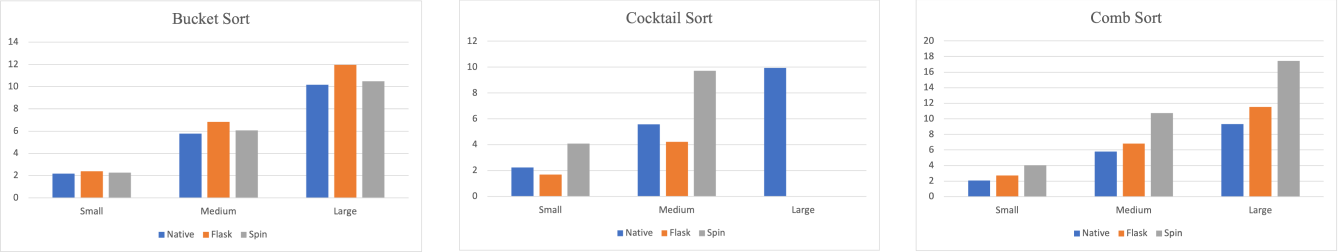
\includegraphics[scale=0.33]{sort2}
\caption{\footnotesize{Benchmark on Bucket Sort, Cocktail Sort and Comb Sort}}
\captionsetup{aboveskip=0pt,font=it}
\end{figure}
\bigskip

\bigskip
\begin{figure}[hp]
\centering
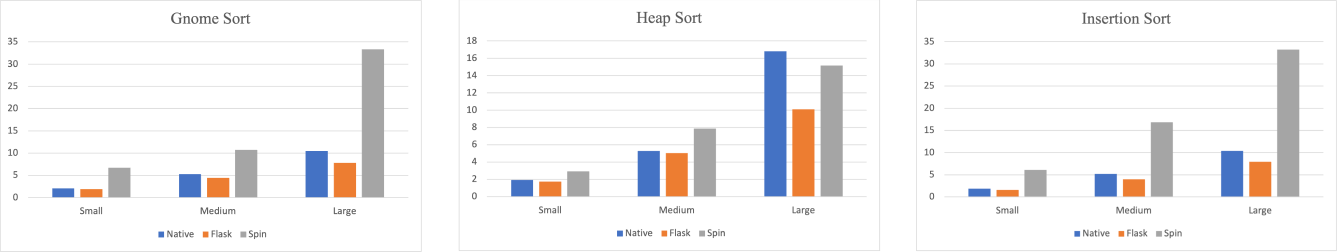
\includegraphics[scale=0.33]{sort3}
\caption{\footnotesize{Benchmark on Gnome Sort, Heap Sort and Insertion Sort}}
\captionsetup{aboveskip=0pt,font=it}
\end{figure}
\bigskip

\bigskip
\begin{figure}[hp]
\centering
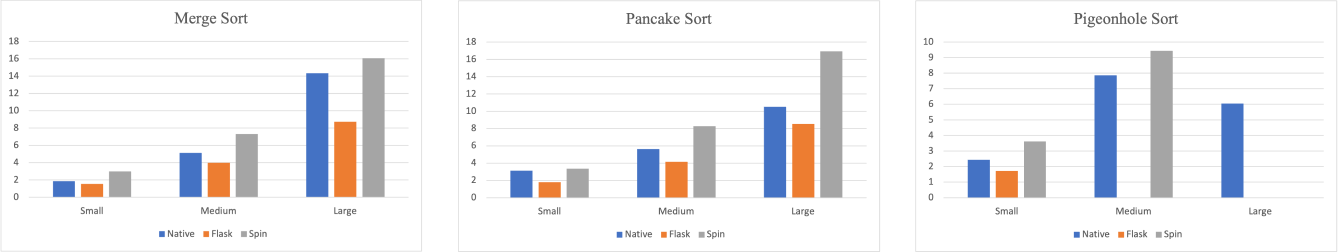
\includegraphics[scale=0.33]{sort4}
\caption{\footnotesize{Benchmark on Merge Sort, Pancake Sort and Pigeonhole Sort}}
\captionsetup{aboveskip=0pt,font=it}
\end{figure}
\bigskip

\newpage
\bigskip
\begin{figure}[hp]
\centering
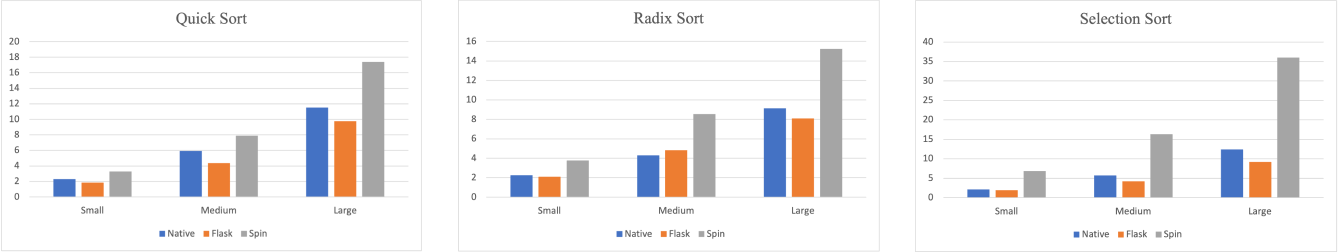
\includegraphics[scale=0.33]{sort5}
\caption{\footnotesize{Benchmark on Quick Sort, Radix Sort and Selection Sort}}
\captionsetup{aboveskip=0pt,font=it}
\end{figure}
\bigskip

\bigskip
\begin{figure}[hp]
\centering
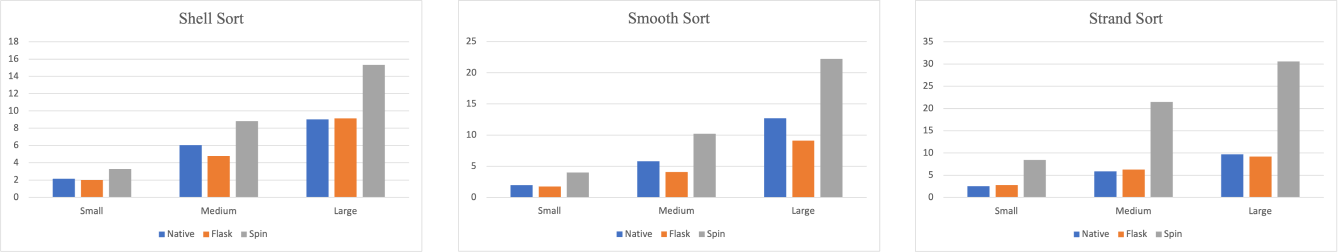
\includegraphics[scale=0.33]{sort6}
\caption{\footnotesize{Benchmark on Shell Sort, Smooth Sort and Strand Sort}}
\captionsetup{aboveskip=0pt,font=it}
\end{figure}
\bigskip

\bigskip
\section{The Outlier}

The outlier here is Bucket Sort. Therefore it is appropriate to list out some of its properties and to form a few hypotheses on the reason behind Spin running faster than Flask executing this algorithm.

We first look at the data input sizes for Bucket Sort with the input array length being \textbf{35000, 55000 and 70000} for small, medium and large, respectively, with the average input length of \textbf{53333}. We do not see this number as an outlier, as other algorithms have a far greater or far smaller average input size. For example, Pigeonhole Sort has an average input array size of \textbf{11666666}, and Brick Sort has an average input array size of \textbf{800}. According to the graph below, Bucket Sort's average array input size is somewhere in the middle across all sorting algorithms.

However, if we remove the \textbf{top two} algorithms with the largest average input array size, we will see a far more average graph with around half \textbf{(7)} of the algorithms having an average input size between \textbf{200000} and \textbf{1000000} (second graph below).

\newpage
\bigskip
\begin{figure}[hp]
\centering
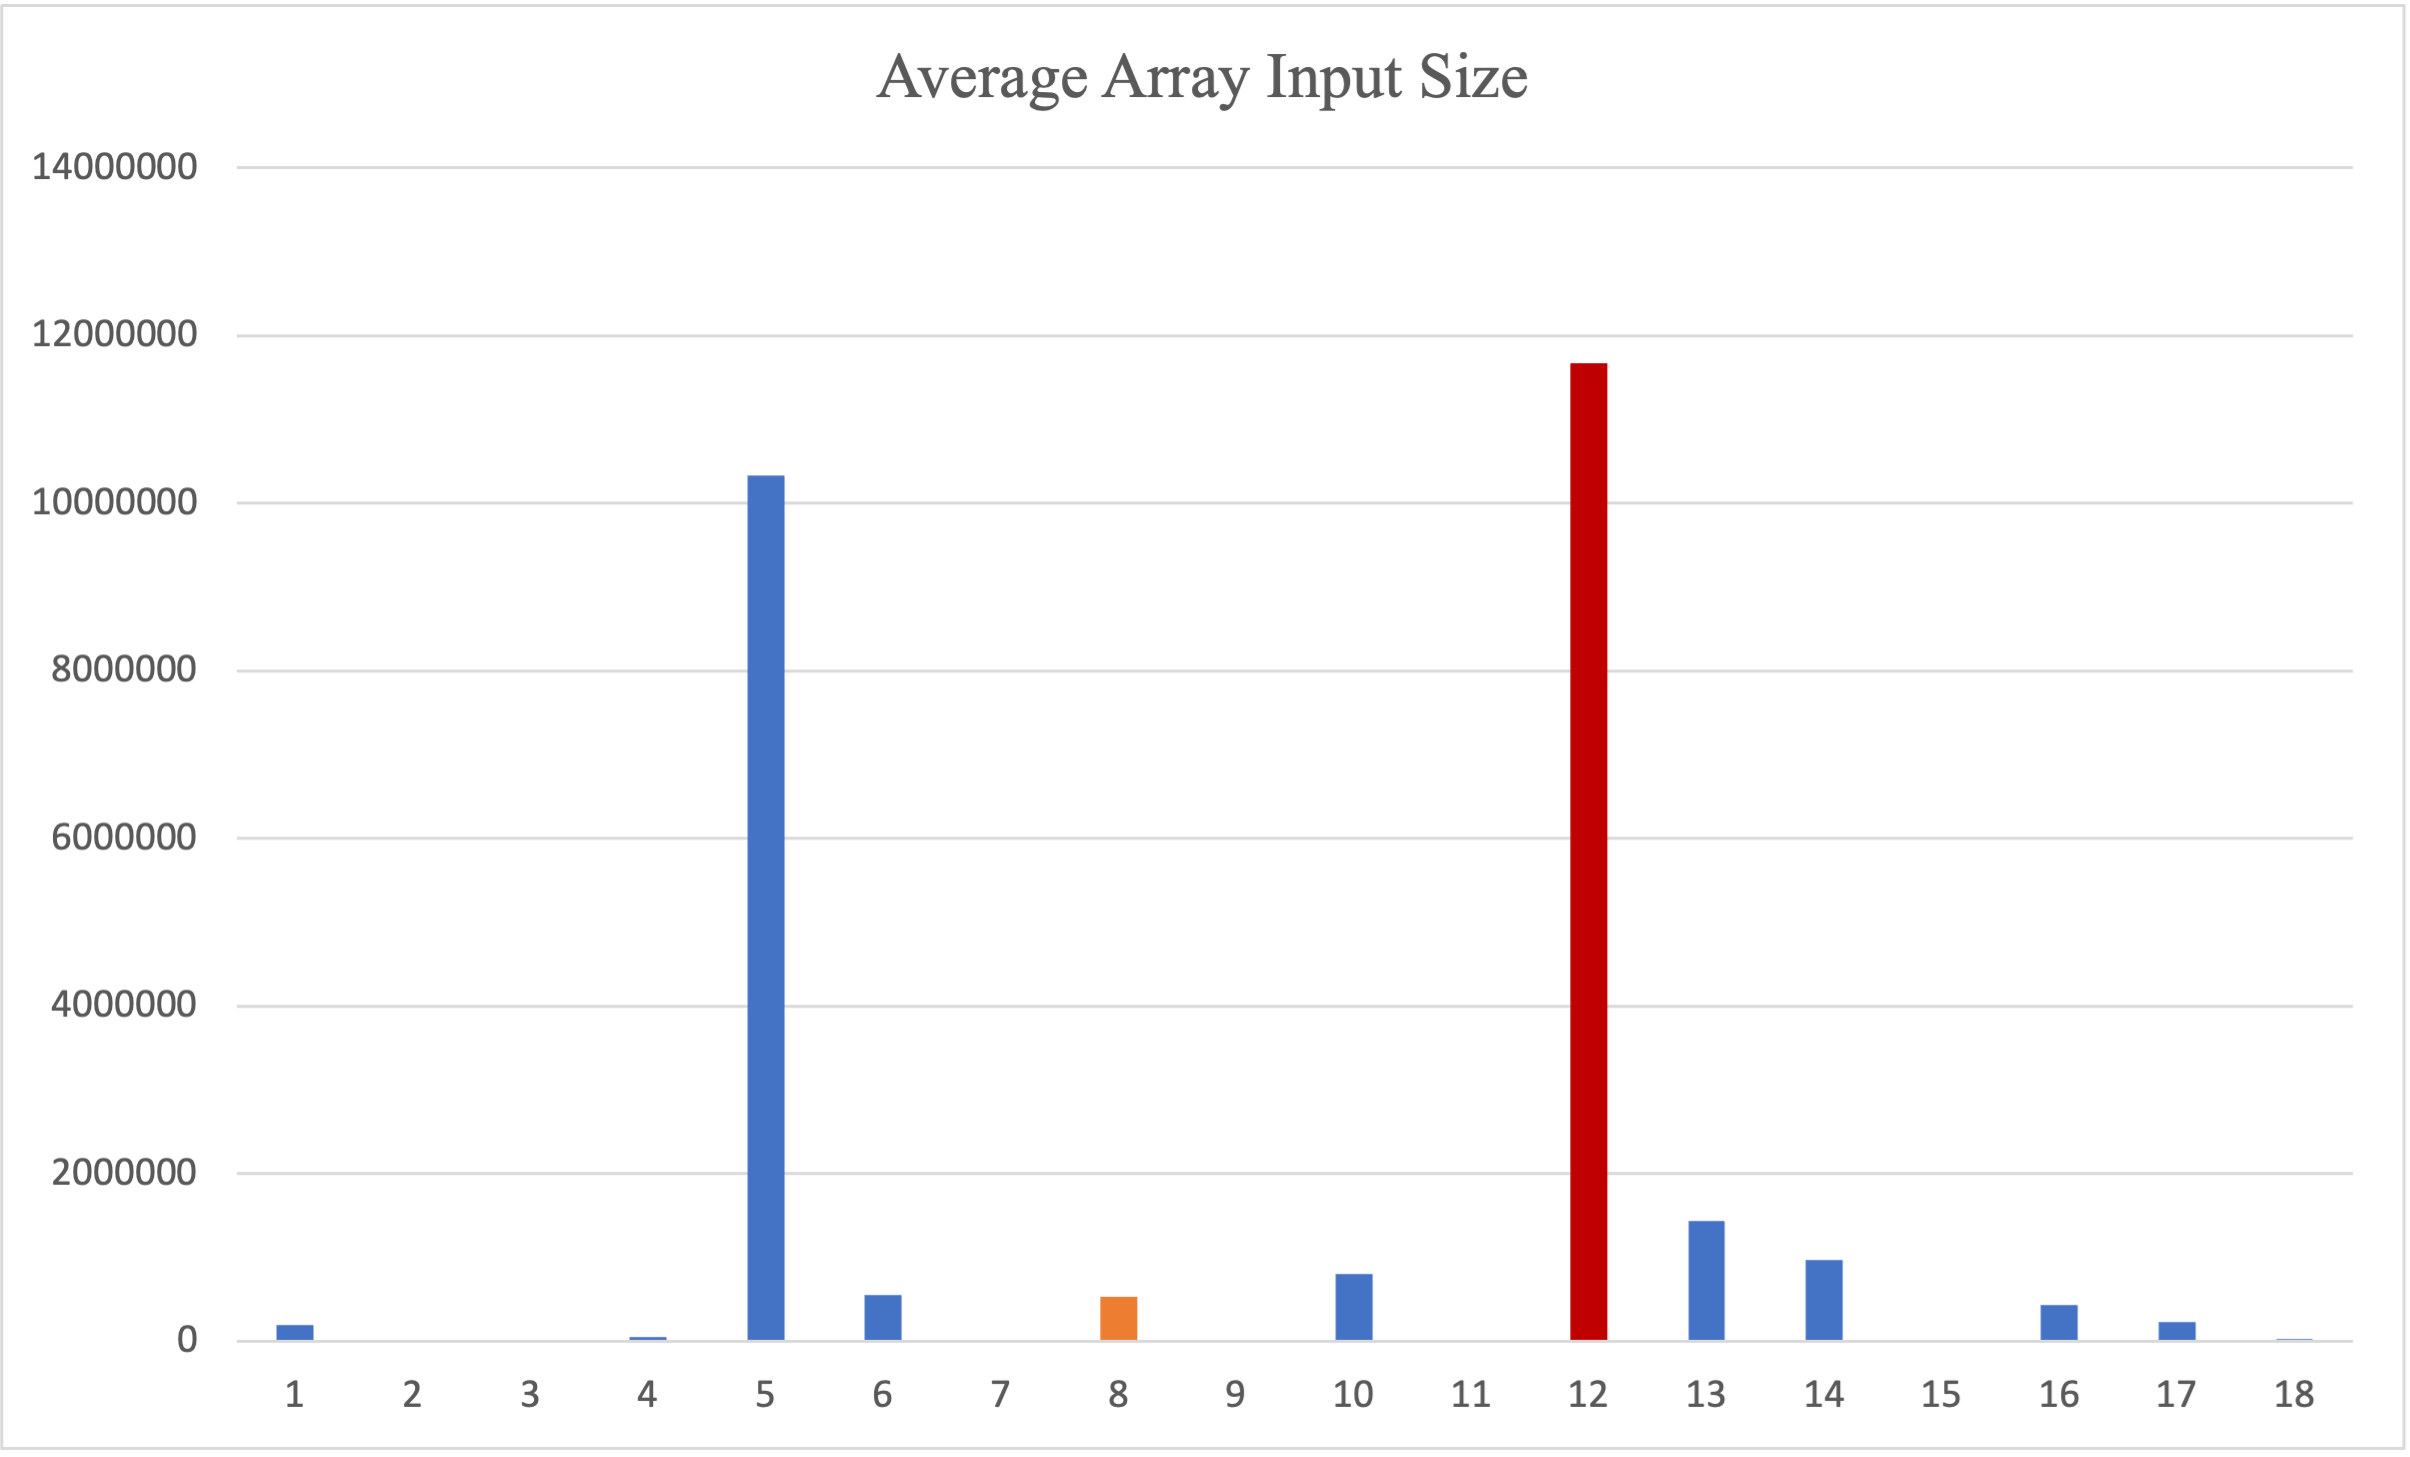
\includegraphics[scale=0.7]{average-sorting-size}
\caption{\footnotesize{Average array input size for all algorithms, green is Brick Sort (non-visible), orange is Bucket Sort, and red is Pigeonhole Sort}}
\captionsetup{aboveskip=0pt,font=it}
\end{figure}
\bigskip

\bigskip
\begin{figure}[hp]
\centering
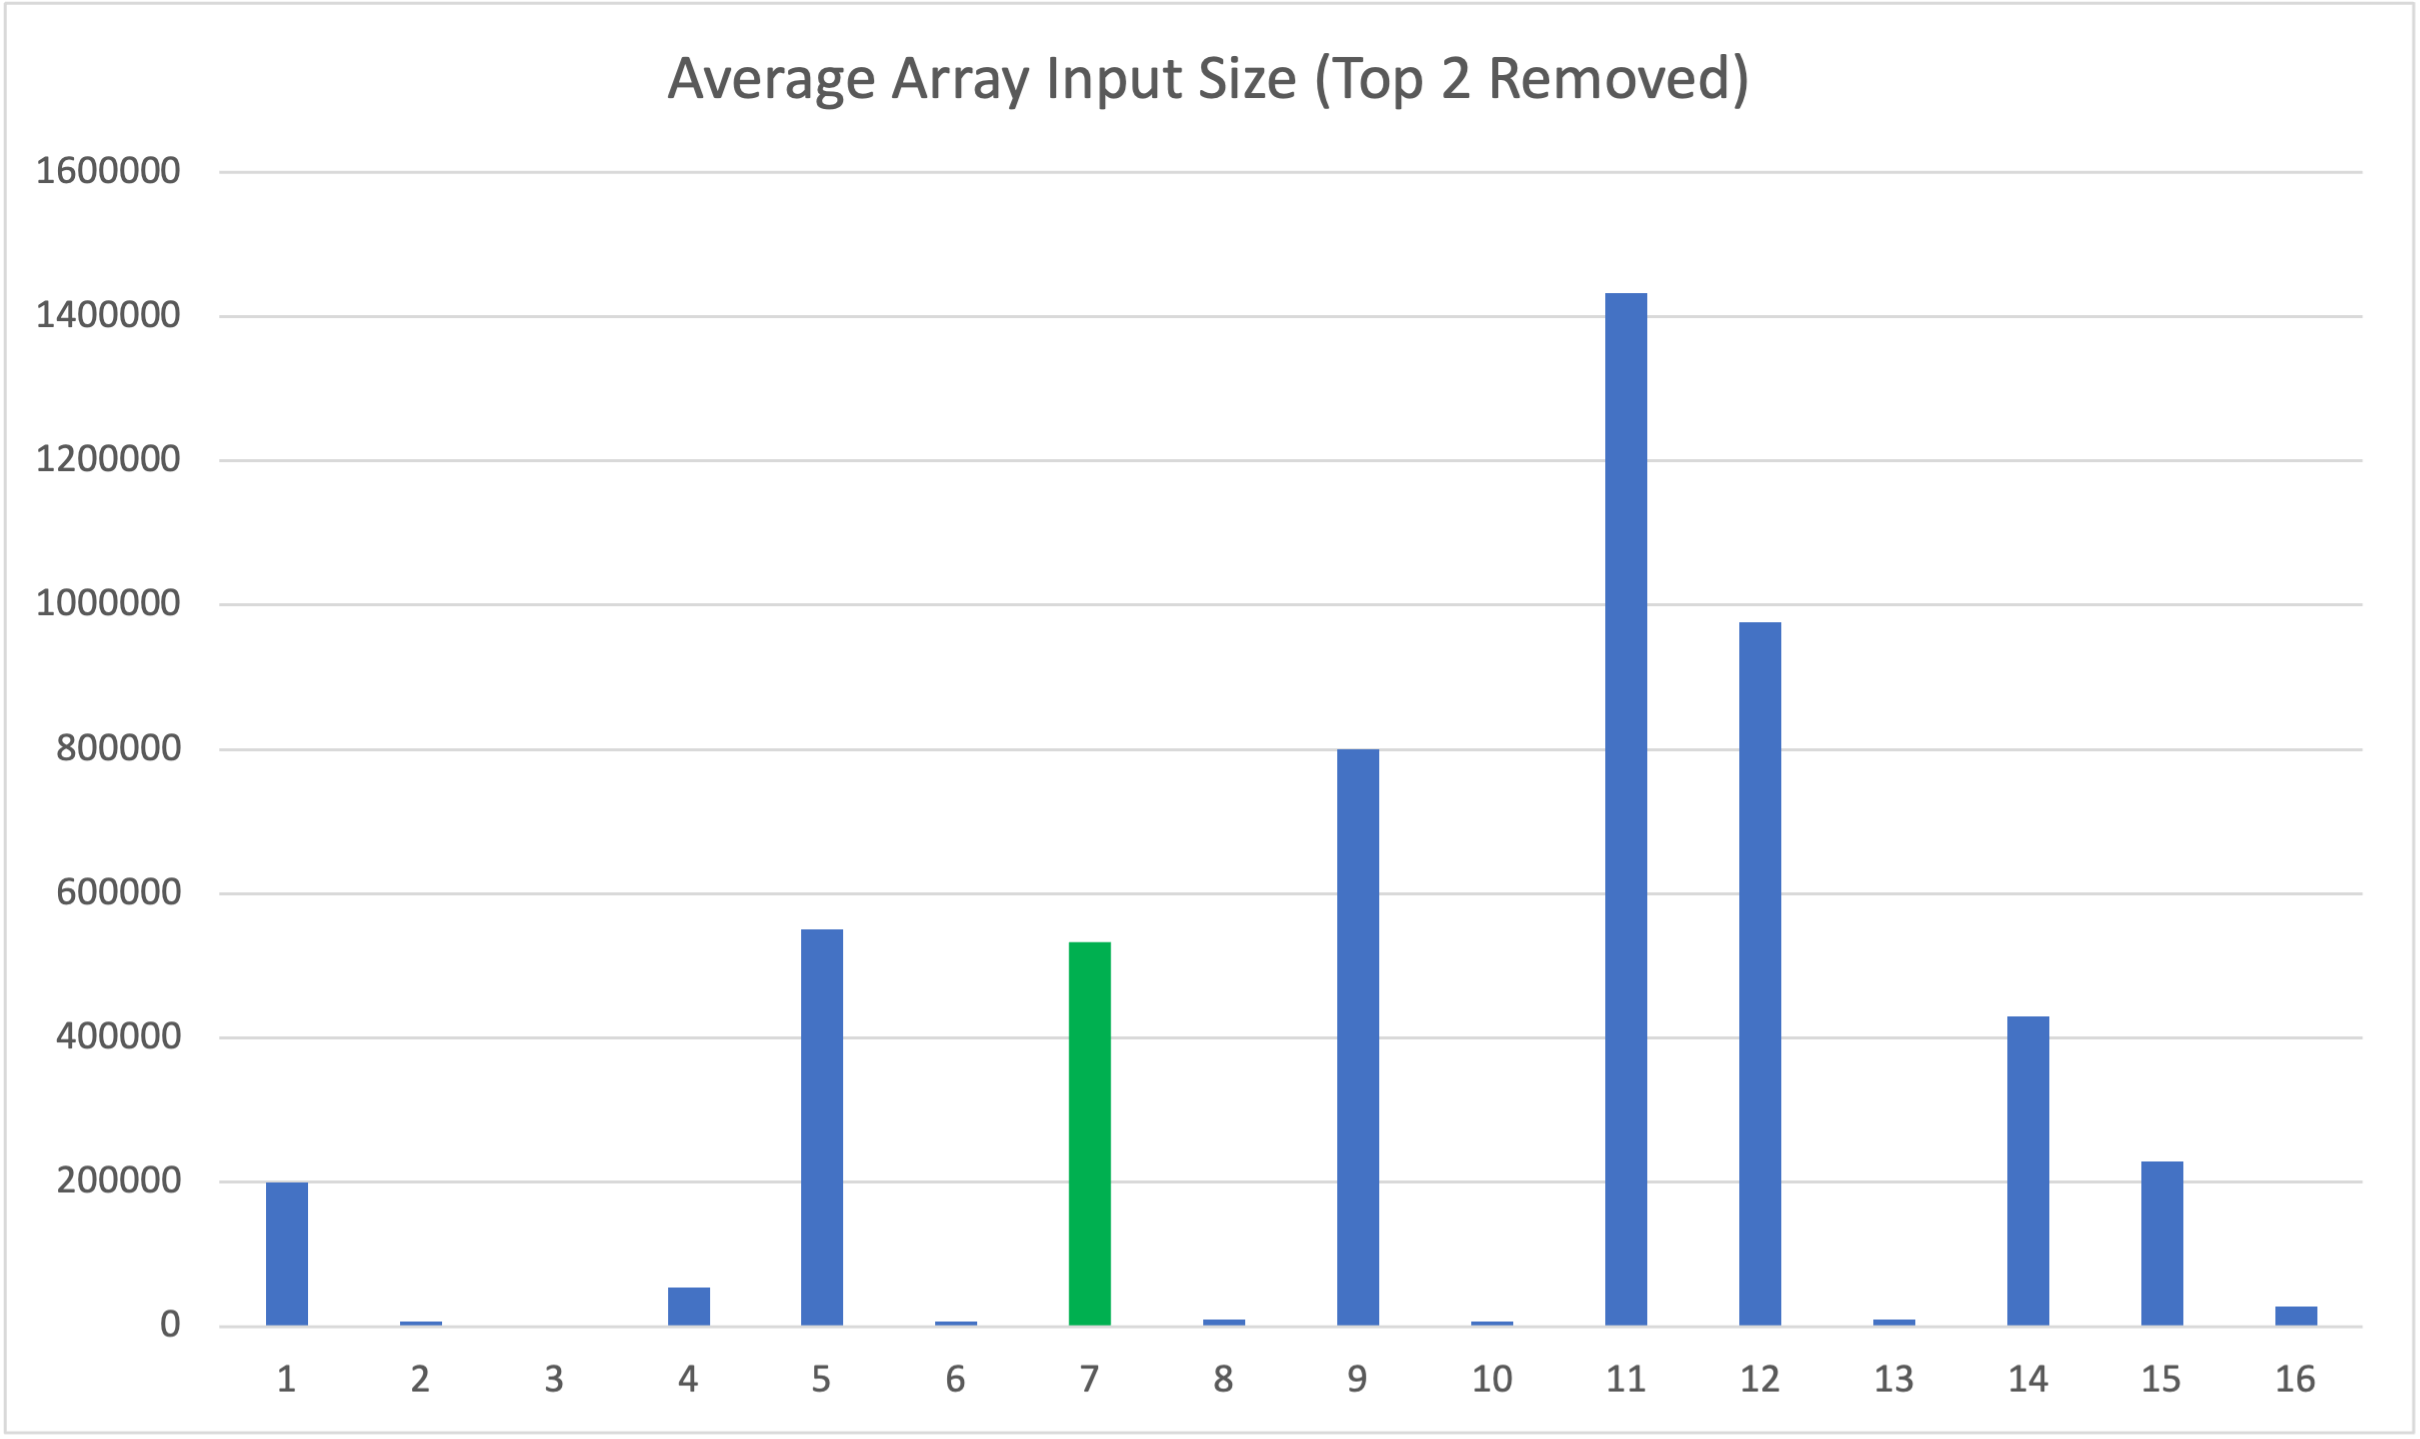
\includegraphics[scale=0.7]{average-sorting-size-2-removed}
\caption{\footnotesize{Average array input size for our sorting algorithm collection with top 2 removed}}
\captionsetup{aboveskip=0pt,font=it}
\end{figure}
\bigskip

We conclude that the input size is not a factor here; therefore, we continue to explore and find out the potential factor behind the performance inconsistency on both frameworks for Bucket Sort.

We then move on to the space complexity for Bucket Sort. As well as addressing the concept behind the algorithm. The space complexity for Bucket Sort is \(n + k\) on average, with the worst space complexity being \(\theta(n\ \cdot\ k)\), where \(n\) is the number of elements in the array and \(k\) is the number of "buckets" used during the sorting process. After adding all elements to \(k\) number of buckets, it will then sort each \(k\) bucket individually with Insertion Sort, which has a space complexity of \(O(1)\).

\bigskip
\begin{figure}[hp]
\centering
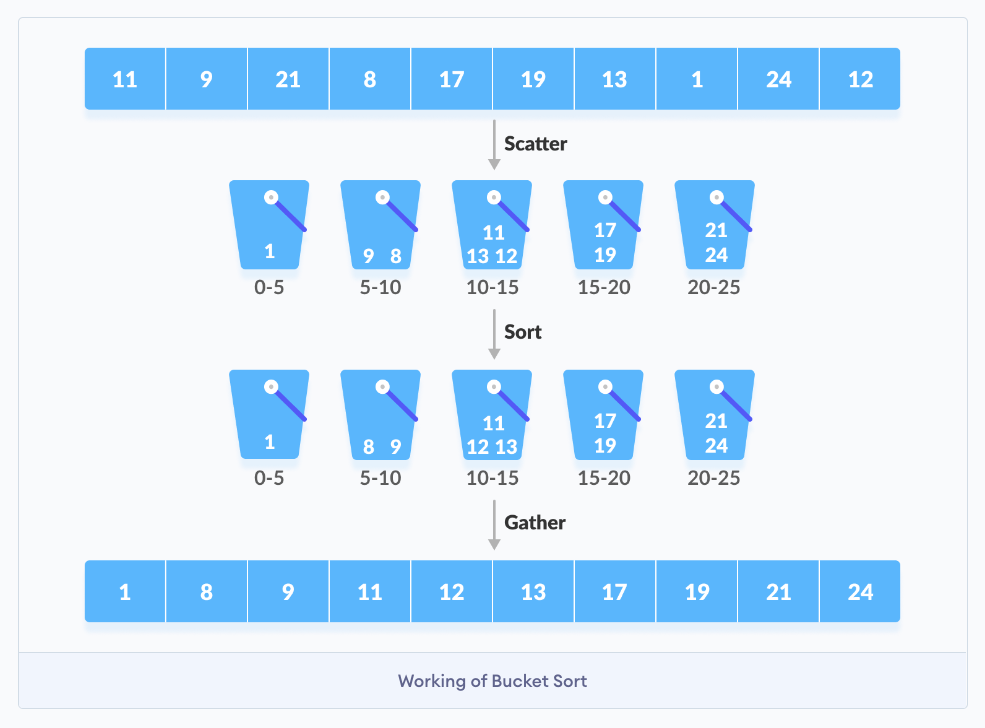
\includegraphics[scale=0.4]{bucket-proz}
\caption{\footnotesize{Working of Bucket Sort \cite{res1}}}
\captionsetup{aboveskip=0pt,font=it}
\end{figure}
\bigskip

From the above figure, we presented the workflow concept for Bucket Sort. At the same time, we recognise that the number of buckets \(k\) can be very different based on the input array. This adds inconsistency to its space complexity, and because of the "bucket" concept used in the algorithm, it uses more memory than any other algorithms in our collection.

Thus, we believe this to be the reason why the Flask framework performs worse than the Spin framework when running Bucket Sort on the input arrays. Especially when running on resource-constraint devices such as the Amazon t3 micro machine, which we introduced in the previous section. On the other hand, WebAssembly has the excellent ability to manage memory usage, and it has clearly shown in this case. Also, note that running this algorithm natively has better performance due to the machine it's running on (2017 MacBook Pro) having a far superior CPU and larger memory.

\bigskip
\section{The Elephant in the Room}

\subsection{Flask vs. Spin}

Except for Bucket Sort, the Flask framework outperformed Spin in 17 out of 18 sorting benchmarks. It was a bit of a surprise when we first recorded the result, and therefore, we ran all experiments 5 times and took the average runtime just to be absolutely sure that the results we were getting from the experiment were consistent. On average, for 17 out of 18 algorithms where Flask outperformed Spin, it ran faster by \textbf{139.212\%} with the lowest runtime increase being \textbf{36.992\%} and the highest being \textbf{309.957\%}.

\bigskip
\begin{figure}[hp]
\centering
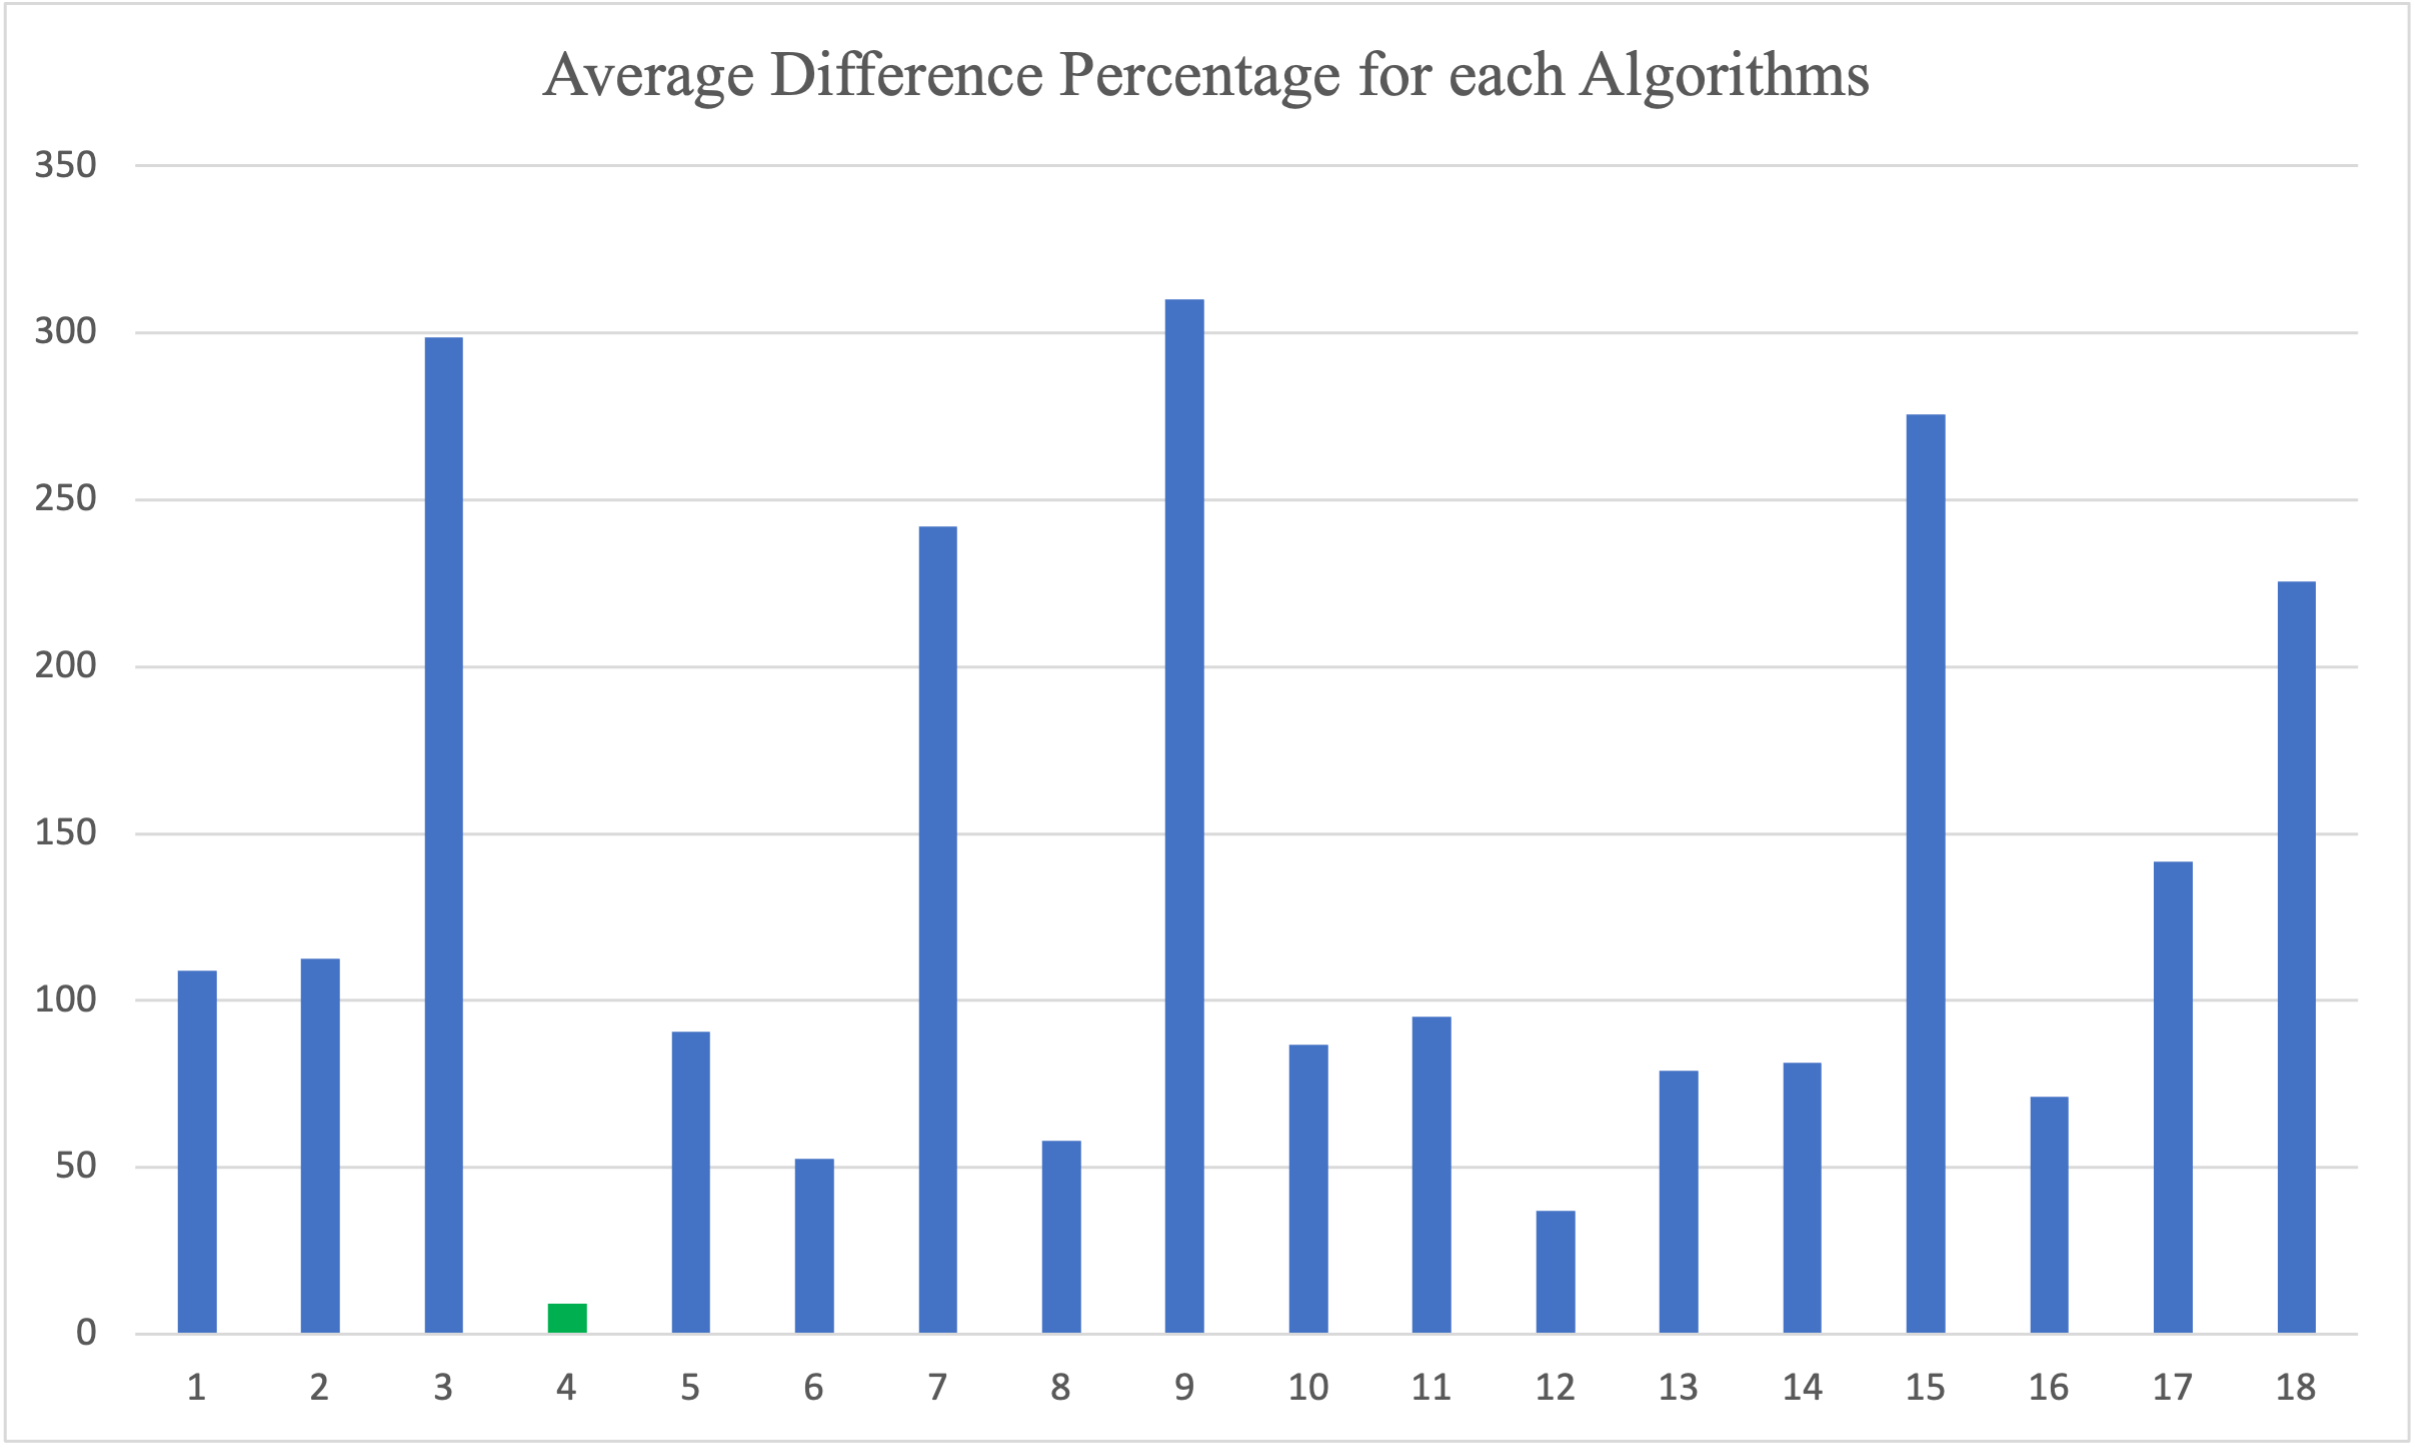
\includegraphics[scale=0.7]{avg-sorting-per}
\caption{\footnotesize{Average performance difference between Flask and Spin, Bucket Sort where Spin outperformed Flask is marked green}}
\captionsetup{aboveskip=0pt,font=it}
\end{figure}
\bigskip

We kept exploring further, and we found that there could be a correlation between the array input size with the average algorithm performance difference. The algorithms with the highest performance differences are \textbf{Brick Sort}, \textbf{Gnome Sort}, \textbf{Insertion Sort}, \textbf{Selection Sort} and \textbf{Strand Sort}. At the same time, they also have some of the smallest array input sizes. In contrast, the \textbf{mean} and the \textbf{medium} for the algorithm performance difference are \textbf{329685.19} and \textbf{126666.5}, respectively. \textbf{Brick Sort} has an average array input size of \textbf{800}, which is way lower than both the mean and the medium. This is also the case with all 4 other algorithms. In fact, \textbf{Brick Sort} and \textbf{Gnome Sort} have the two lowest array input size out of all \textbf{18} algorithms \textbf{(800 and 6500)}, while \textbf{Selection Sort} has the \textbf{fifth} lowest array input size \textbf{(9833)}, \textbf{Insertion Sort} \textbf{sixth} \textbf{(10000)}, and \textbf{Strand Sort}, \textbf{seventh} \textbf{(28333)}.

\bigskip
\begin{figure}[hp]
\centering
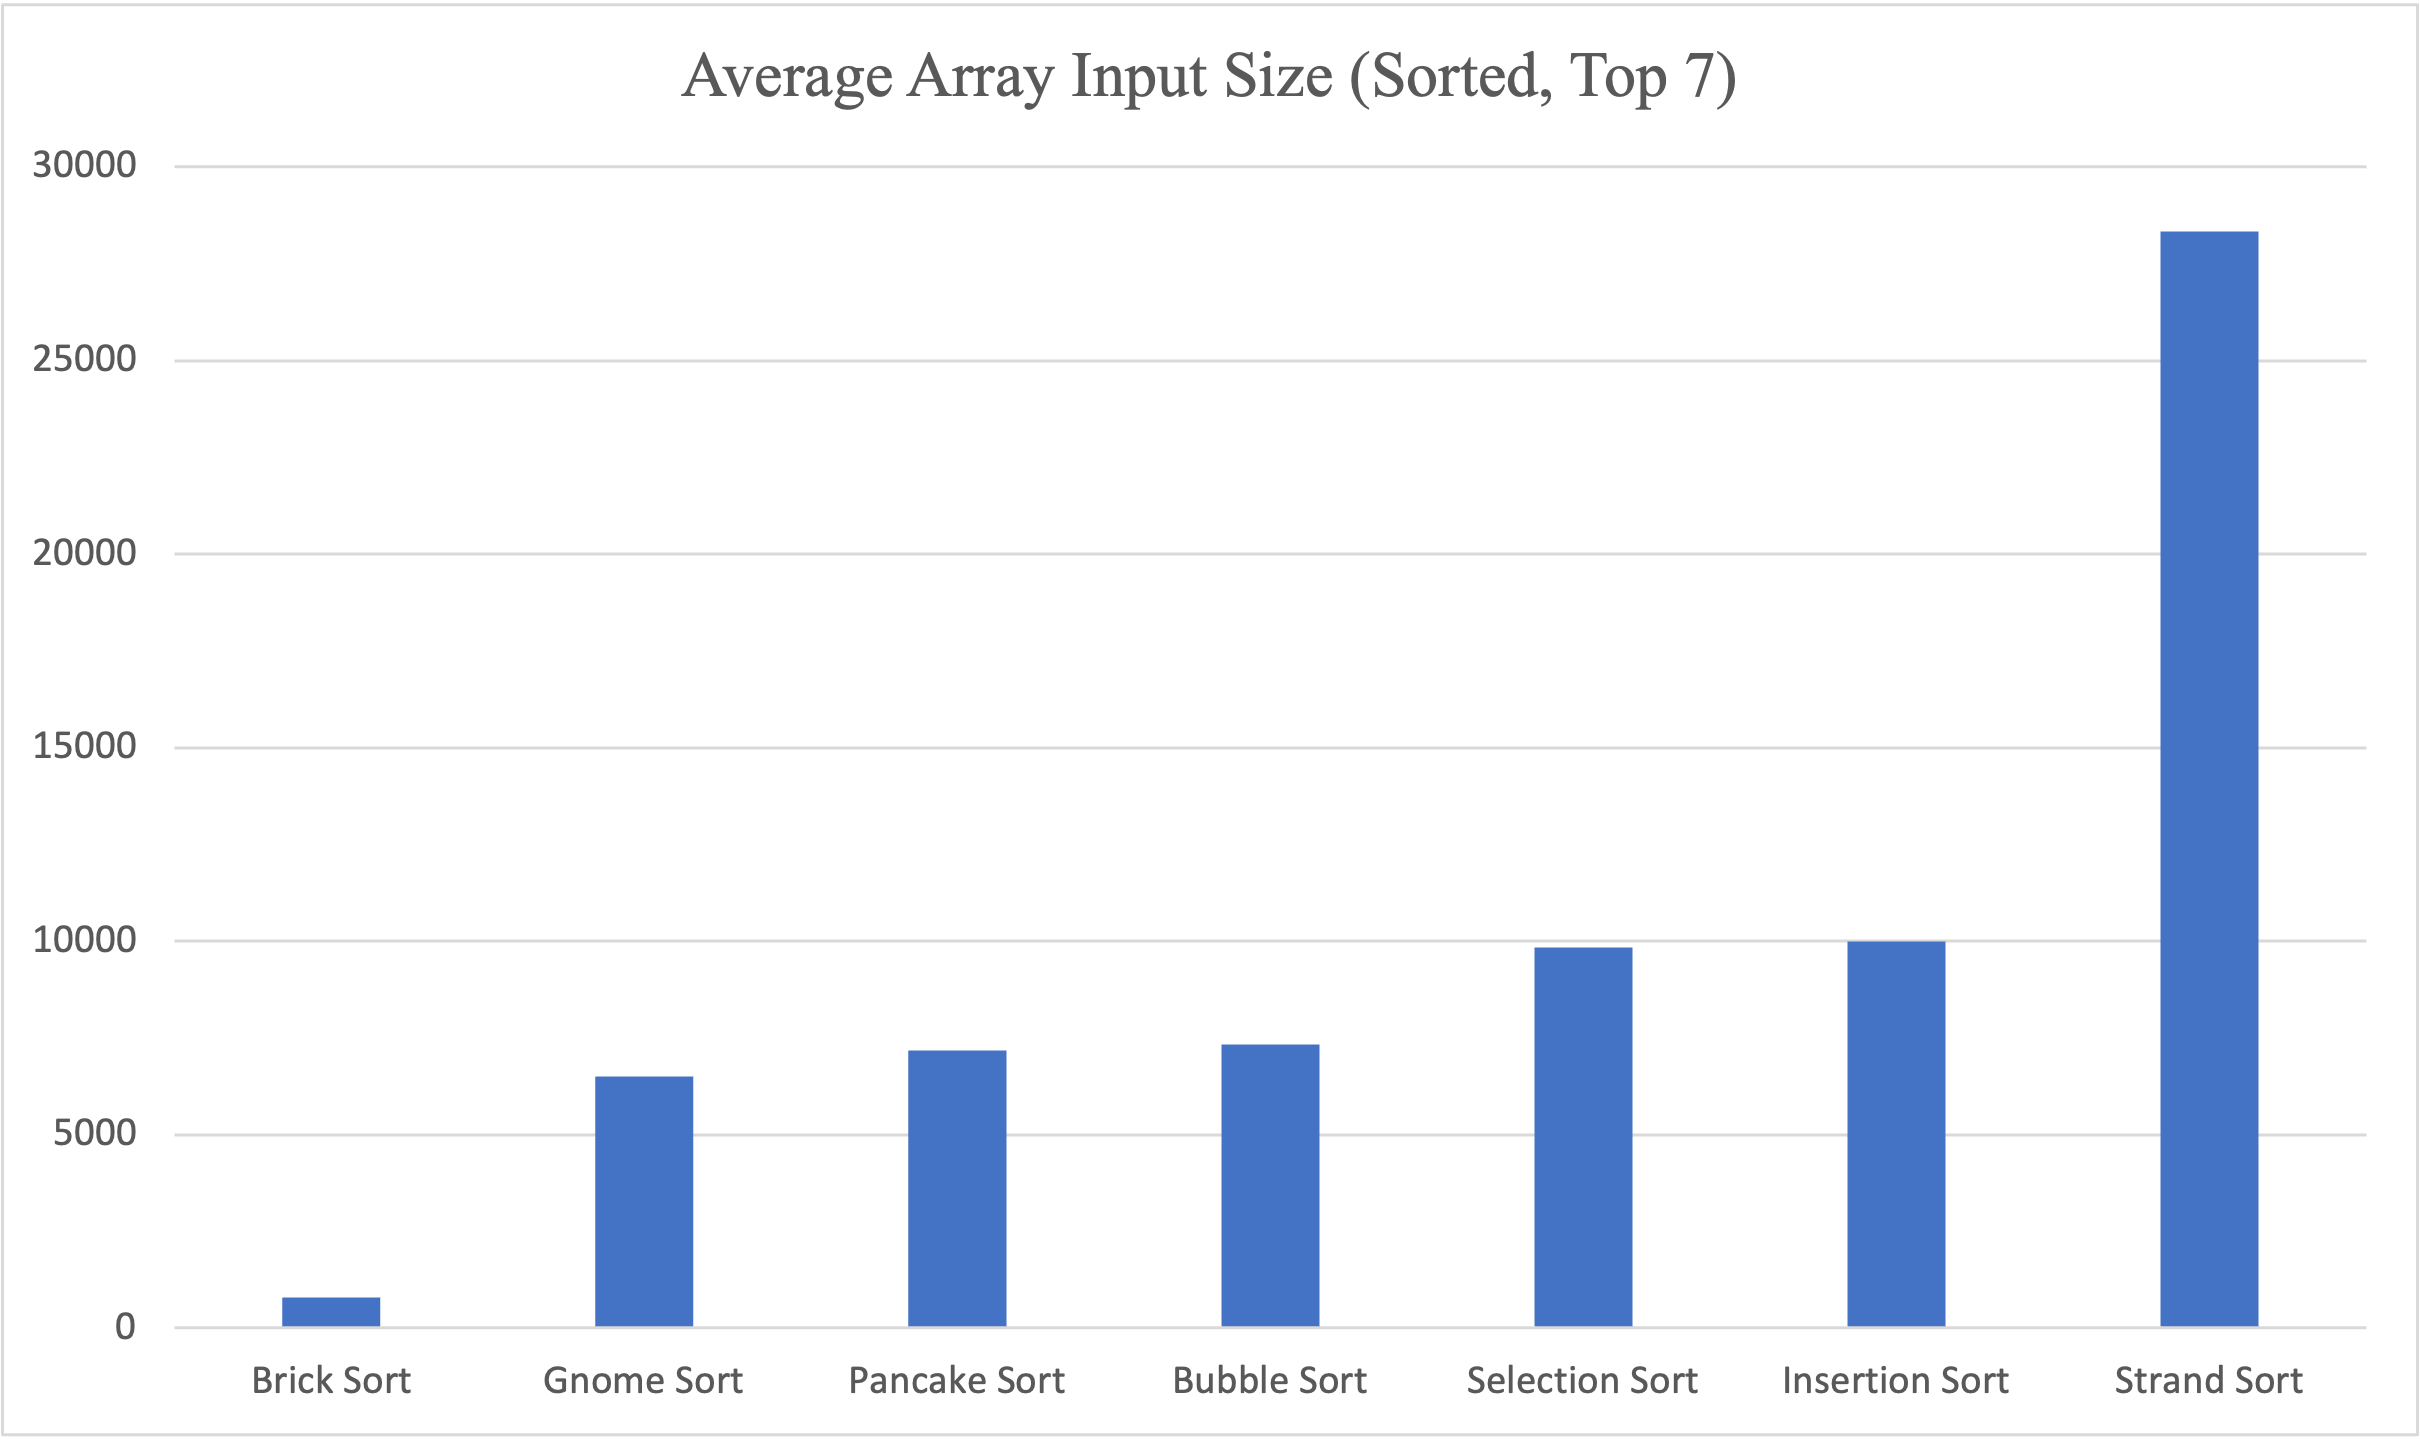
\includegraphics[scale=0.7]{avg-sorting-per-sorted-7}
\caption{\footnotesize{Average array input size (Sorted from lowest to highest, Top 7)}}
\captionsetup{aboveskip=0pt,font=it}
\end{figure}
\bigskip

\subsection{Native Environment vs. Flask}

We also noticed that the Flask framework outperformed the Native Environment from time to time. Across \textbf{18} benchmarks and \textbf{51} valid tests where both Native and Flask runtime data were recorded successfully, Native only outperformed Flask \textbf{10} times, or \textbf{19.6\%} of time.

Ahead of the experiment, we believe benchmarks running on a native environment will perform best since it has little overhead as well as more CPU and memory resources than running in a cloud or edge environment. However, we believe this inconsistency is due to the continuous development, optimisation and integration with Python on the Flask framework, which was initially released back in 2010.

\bigskip
\section{Further Exploring with Standard Deviation}

As stated above, we run each benchmark \textbf{5} times to ensure the result data is consistent. We calculate the standard deviation for \textbf{5} benchmarks \textbf{(Quick Sort, Merge Sort, Selection Sort, Insertion Sort and Bubble Sort)} to ensure runtime from each iteration does not spread out too much.

\bigskip
\begin{table}[h!]
\centering
\begin{tabular}{||c c c c||} 
\hline
Name & Standard Deviation ($\sigma$) & Confidence Interval & 95\% Confidence Interval \\ [1ex] 
\hline\hline
 & & & \\
Quick Sort (S) & 0.16 & 0.071 & 1.8424 ±0.14 (±7.62\%) \\
 & & & \\
Quick Sort (M) & 0.17 & 0.075 & 4.3692 ±0.146 (±3.35\%) \\
 & & & \\
Quick Sort (L) & 0.436 & 0.195 & 9.7668 ±0.382 (±3.91\%) \\
 & & & \\
Merge Sort (S) & 0.045 & 0.02 & 1.5396 ±0.0395 (±2.56\%) \\
 & & & \\
Merge Sort (M) & 0.13 & 0.058 & 3.9864 ±0.114 (±2.86\%) \\
 & & & \\
Merge Sort (L) & 0.416 & 0.186 & 8.7294 ±0.365 (±4.18\%) \\
 & & & \\
Selection Sort (S) & 0.154 & 0.069 & 1.9406 ±0.135 (±6.97\%) \\
 & & & \\
Selection Sort (M) & 0.188 & 0.084 & 4.2406 ±0.165 (±3.88\%) \\
 & & & \\
Selection Sort (L) & 0.144 & 0.064 & 9.2008 ±0.126 (±1.37\%) \\
 & & & \\
Insertion Sort (S) & 0.143 & 0.064 & 1.5734 ±0.125 (±7.97\%) \\
 & & & \\
Insertion Sort (M) & 0.264 & 0.118 & 3.9772 ±0.231 (±5.81\%) \\
 & & & \\
Insertion Sort (L) & 0.437 & 0.195 & 7.9312 ±0.383 (±4.83\%) \\
 & & & \\
Bubble Sort (S) & 0.021 & 0.009 & 2.167 ±0.0187 (±0.86\%) \\
 & & & \\
Bubble Sort (M) & 0.149 & 0.067 & 4.4062 ±0.13 (±2.96\%) \\
 & & & \\
Bubble Sort (L) & 0.605 & 0.27 & 9.2836 ±0.53 (±5.71\%) \\ [1ex]
\hline
\end{tabular}
\caption{Standard deviation for Flask framework}
\label{table:time_complexity_2}
\end{table}
\bigskip

\bigskip
\begin{table}[h!]
\centering
\begin{tabular}{||c c c c||} 
\hline
Name & Standard Deviation ($\sigma$) & Confidence Interval & 95\% Confidence Interval \\ [1ex] 
\hline\hline
 & & & \\
Quick Sort (S) & 0.111 & 0.05 & 3.2788 ±0.0975 (±2.97\%) \\
 & & & \\
Quick Sort (M) & 0.214 & 0.075 & 0.096 ±0.187 (±2.37\%) \\
 & & & \\
Quick Sort (L) & 0.5 & 0.222 & 17.3986 ±0.436 (±2.50\%) \\
 & & & \\
Merge Sort (S) & 0.253 & 0.113 & 2.9772 ±0.221 (±7.43\%) \\
 & & & \\
Merge Sort (M) & 0.314 & 0.14 & 7.3058 ±0.275 (±3.77\%) \\
 & & & \\
Merge Sort (L) & 0.9 & 0.402 & 16.0678 ±0.789 (±4.91\%) \\
 & & & \\
Selection Sort (S) & 0.307 & 0.137 & 6.8086 ±0.269 (±3.96\%) \\
 & & & \\
Selection Sort (M) & 0.532 & 0.238 & 16.3238 ±0.466 (±2.86\%) \\
 & & & \\
Selection Sort (L) & 0.759 & 0.339 & 35.981 ±0.665 (±1.85\%) \\
 & & & \\
Insertion Sort (S) & 0.069 & 0.03 & 6.096 ±0.0603 (±0.99\%) \\
 & & & \\
Insertion Sort (M) & 0.306 & 0.137 & 16.8586 ±0.268 (±1.59\%) \\
 & & & \\
Insertion Sort (L) & 0.909 & 0.407 & 33.196 ±0.797 (±2.40\%) \\
 & & & \\
Bubble Sort (S) & 0.343 & 0.154 & 8.8656 ±0.301 (±3.39\%) \\
 & & & \\
Bubble Sort (M) & 0.335 & 0.15 & 17.7418 ±0.294 (±1.66\%) \\
 & & & \\
Bubble Sort (L) & 0.954 & 0.427 & 35.6476 ±0.837 (±2.35\%) \\ [1ex]
\hline
\end{tabular}
\caption{Standard deviation for Spin framework}
\label{table:time_complexity_2}
\end{table}
\bigskip

We discovered a few interesting things in the above analysis for the standard deviation. First, overall the standard deviation for all benchmarking algorithms with all 3 data input sizes is relatively small. This means the runtime data we get from running the benchmark algorithms each time are fairly consistent and do not spread out too much. Thus, we can be sure that we are confident with the data we analysed using the average runtime data calculated in the earlier section.

The second thing we found is that for both frameworks, we tend to get a larger number of standard deviations than the input data. For example, the average standard deviation for \textbf{small} array input size is \textbf{0.105} for Flask and \textbf{0.217} for Spin. In contrast, the average standard deviation for \textbf{large} array input size is \textbf{0.408} for Flask and \textbf{0.804} for Spin, which is \textbf{3.9 times} and \textbf{3.72 times} greater than their small data input counterpart respectively. This means that the result data spreads wider and less consistent the larger the input data is. This is also an interesting phenomenon that we believe is worthy of further research.

\bigskip
\section{Shortest Path and Minimum Spanning Tree Algorithm Analysis}

The second stage of our experiment is benchmarking an extra \textbf{4} Shortest Path and Minimum Spanning Tree Algorithms. They are \textbf{Dijkstra's algorithm}, \textbf{Floyd–Warshall algorithm}, \textbf{Kruskal's algorithm} and \textbf{Prim's algorithm}.

\subsection{Performances between Flask and Spin}

For all \textbf{4} benchmarking algorithms in the second stage \textbf{(10 valid tests)}, Flask outperformed Spin on every single one of them by an average of \textbf{107.571\%}, with the lowest runtime increase being \textbf{30.224\%} and the highest being \textbf{151.368\%}. On the other hand, the average runtime increase with the \textbf{small} data input size is \textbf{290.322\%}, the \textbf{medium}: \textbf{106.057\%} and the \textbf{large} is \textbf{138.753\%}. With the knowledge from the first experiment, we are not surprised by the results we got from the shortest path and minimum spanning tree algorithms.

Here are the results from stage 2 of the experiment:

\bigskip
\begin{figure}[hp]
\centering
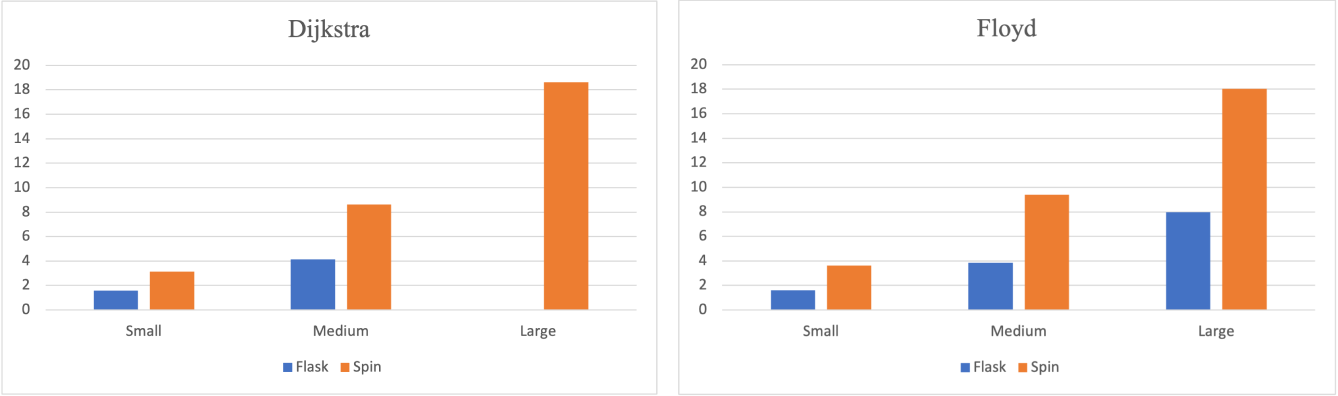
\includegraphics[scale=0.33]{images/other1}
\caption{\footnotesize{Benchmark on Dijkstra and Floyd–Warshall}}
\captionsetup{aboveskip=0pt,font=it}
\end{figure}
\bigskip

\newpage
\bigskip
\begin{figure}[hp]
\centering
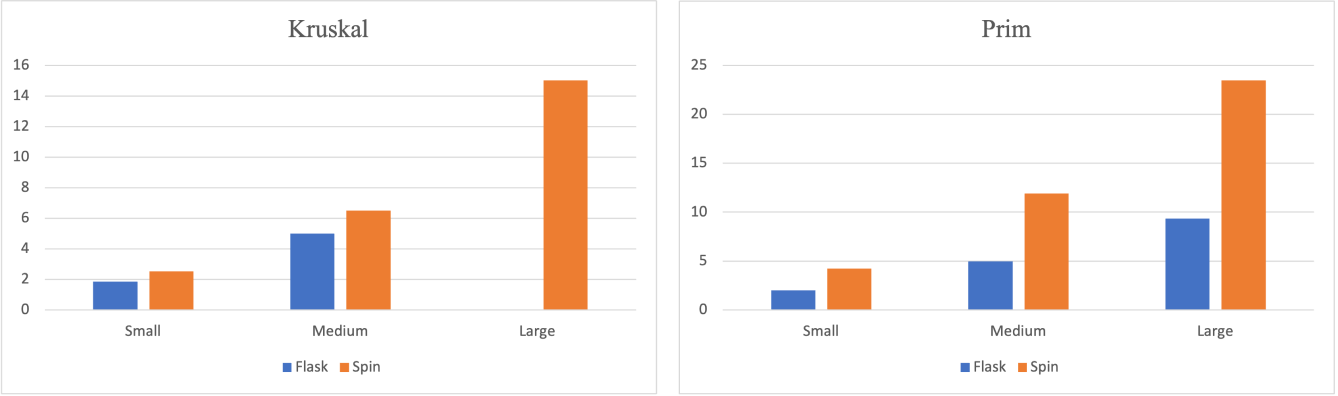
\includegraphics[scale=0.33]{images/other2}
\caption{\footnotesize{Benchmark on Kruskal and Prim}}
\captionsetup{aboveskip=0pt,font=it}
\end{figure}
\bigskip


\subsection{The case of Kruskal's Algorithm}

We further look at the average speed-up percentage per algorithm. For Dijkstra's algorithm, Flask outperformed Spin by \textbf{103.784\%} on average. For Floyd–Warshall, it was \textbf{132.923\%}. Then, Kruskal, \textbf{33.132\%} on average and lastly, Flask outperformed Spin by \textbf{134.369\%} on average running Prim's algorithm.

In the case of Kruskal's algorithm, we discovered that the average speed-up percentage is lower than the other 3 algorithms. In fact, Kruskal's algorithm is the only benchmarking algorithm in our collection where the average speed-up percentage is below 100\%. It is also below the average speed-up percentage across all tests by \textbf{224.679\%}. Within \textbf{8} tests performed across Dijkstra, Floyd and Prim, only \textbf{1} test where the average speed-up rate is below 100 \textbf{(Dijkstra's algorithm with small input data)}.

\newpage
\begin{figure}[hp]
\centering
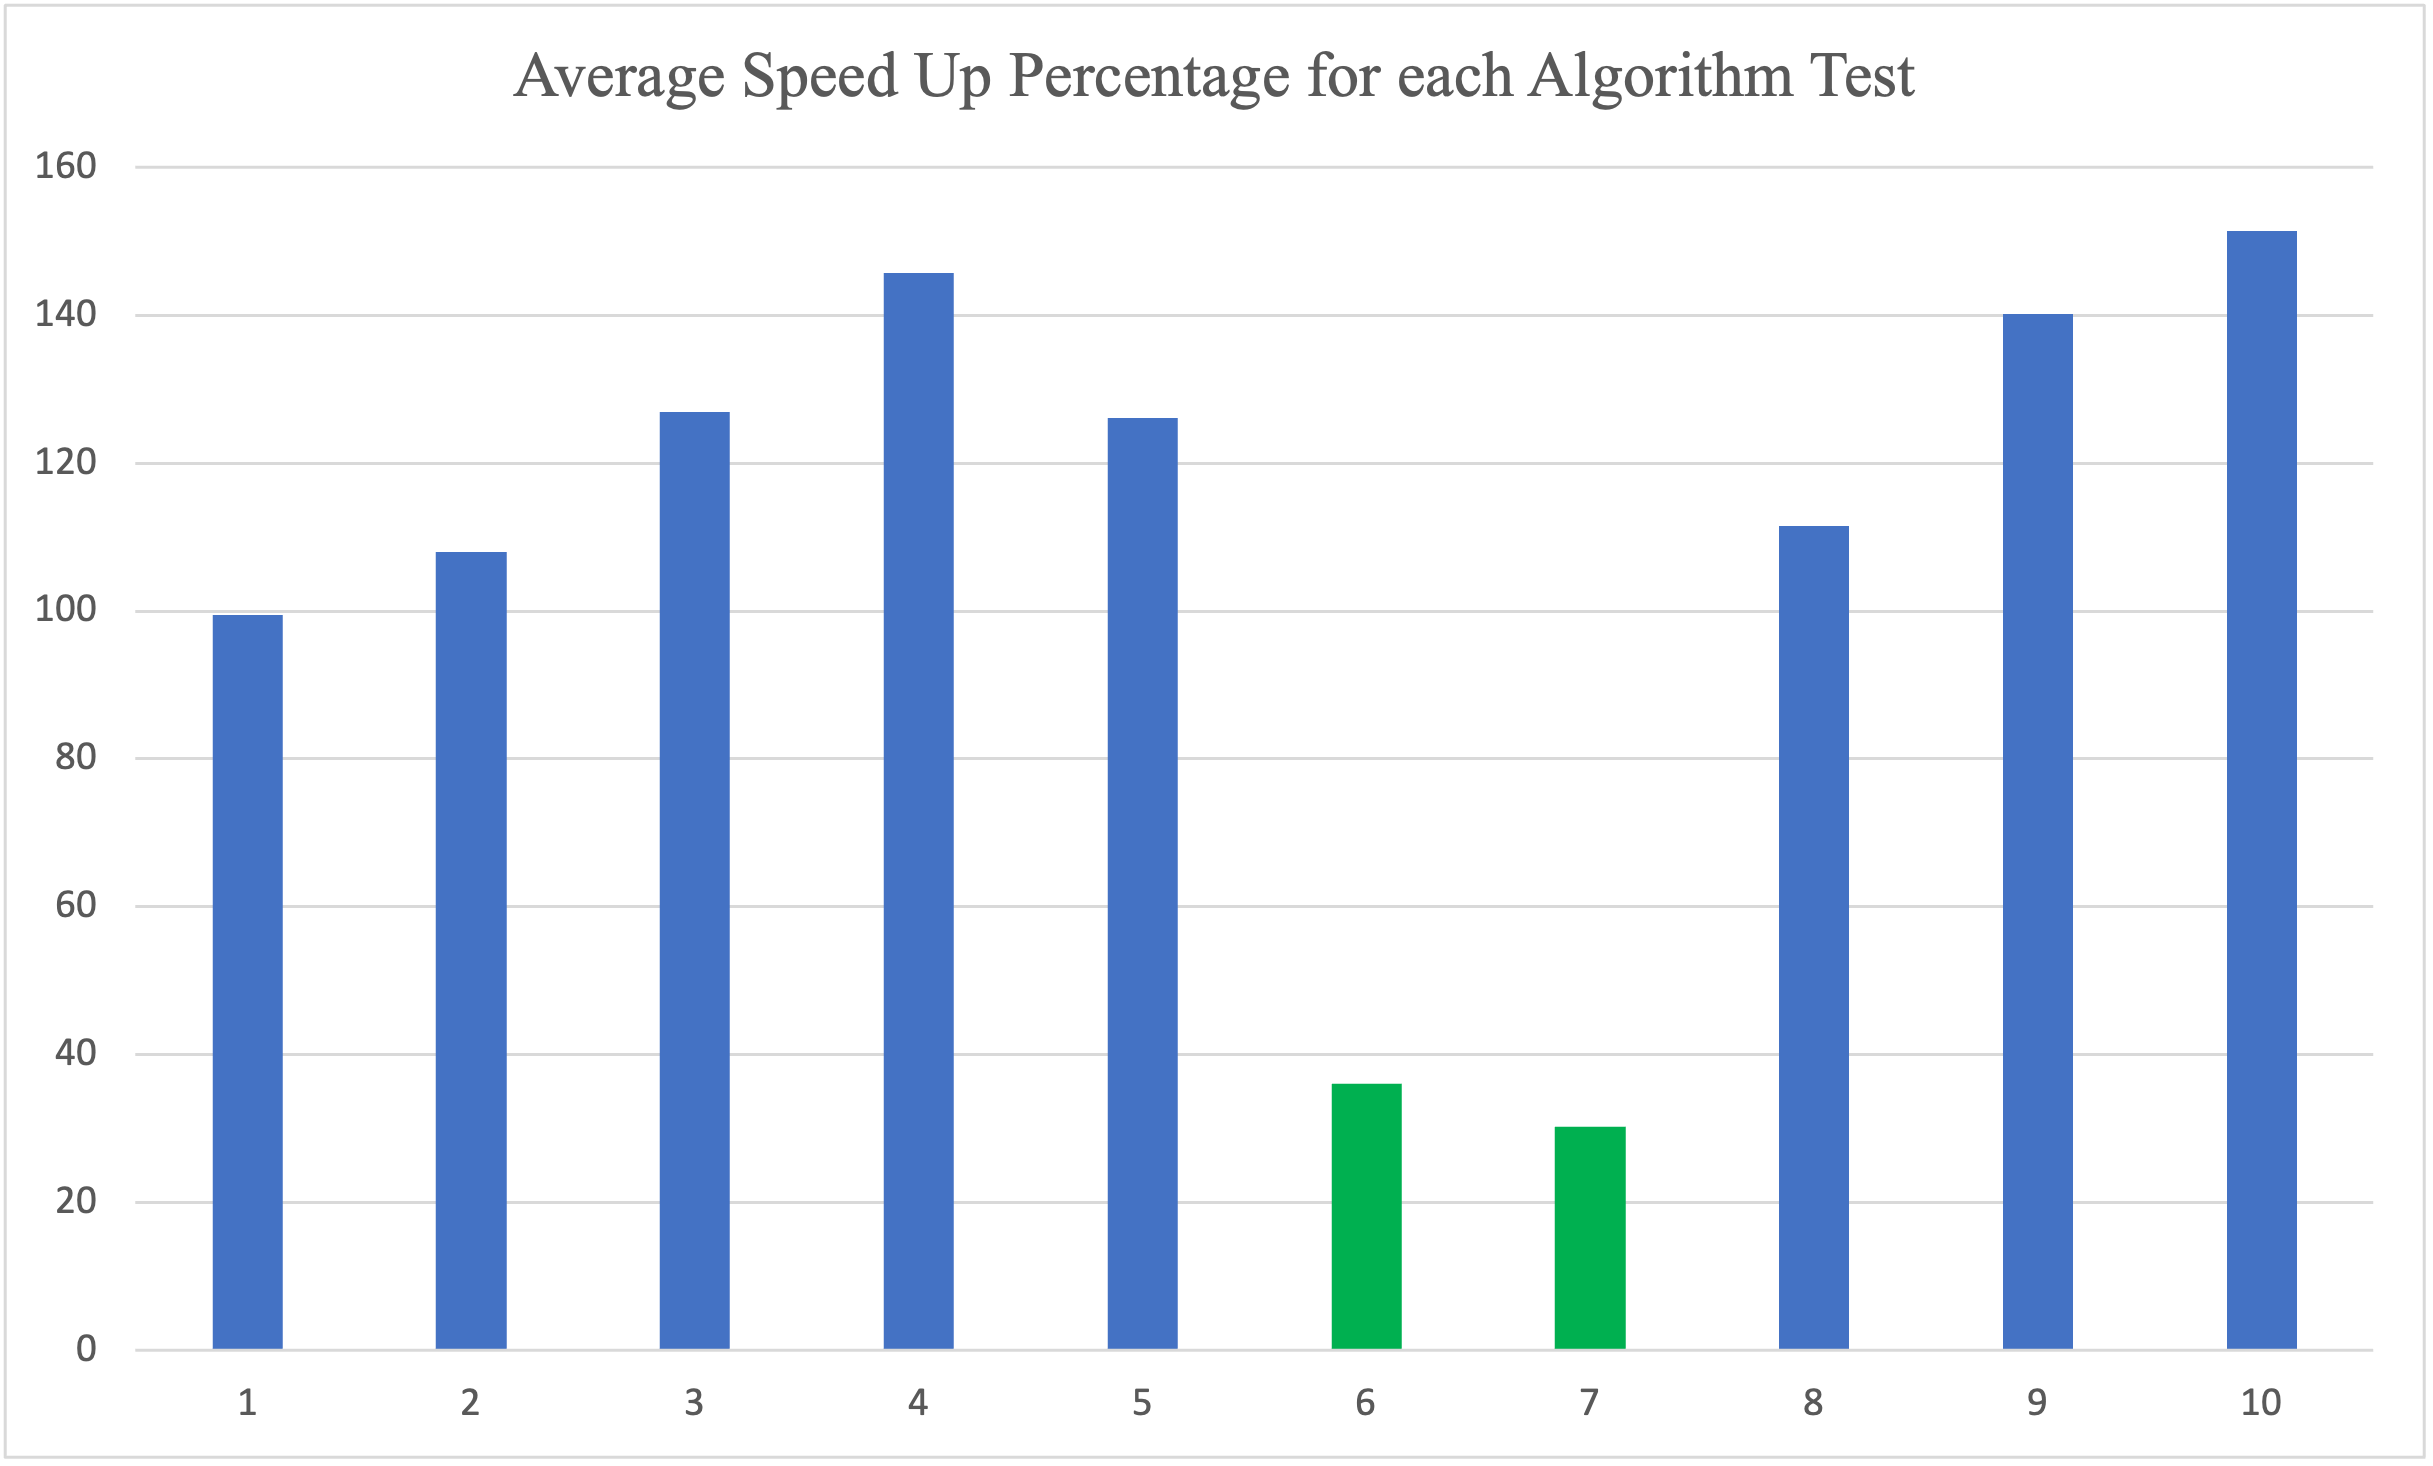
\includegraphics[scale=0.6]{avg-other-per-test}
\caption{\footnotesize{Average performance difference between Flask and Spin on each test, Kruskal is marked green}}
\captionsetup{aboveskip=0pt,font=it}
\end{figure}

\bigskip
\begin{figure}[hp]
\centering
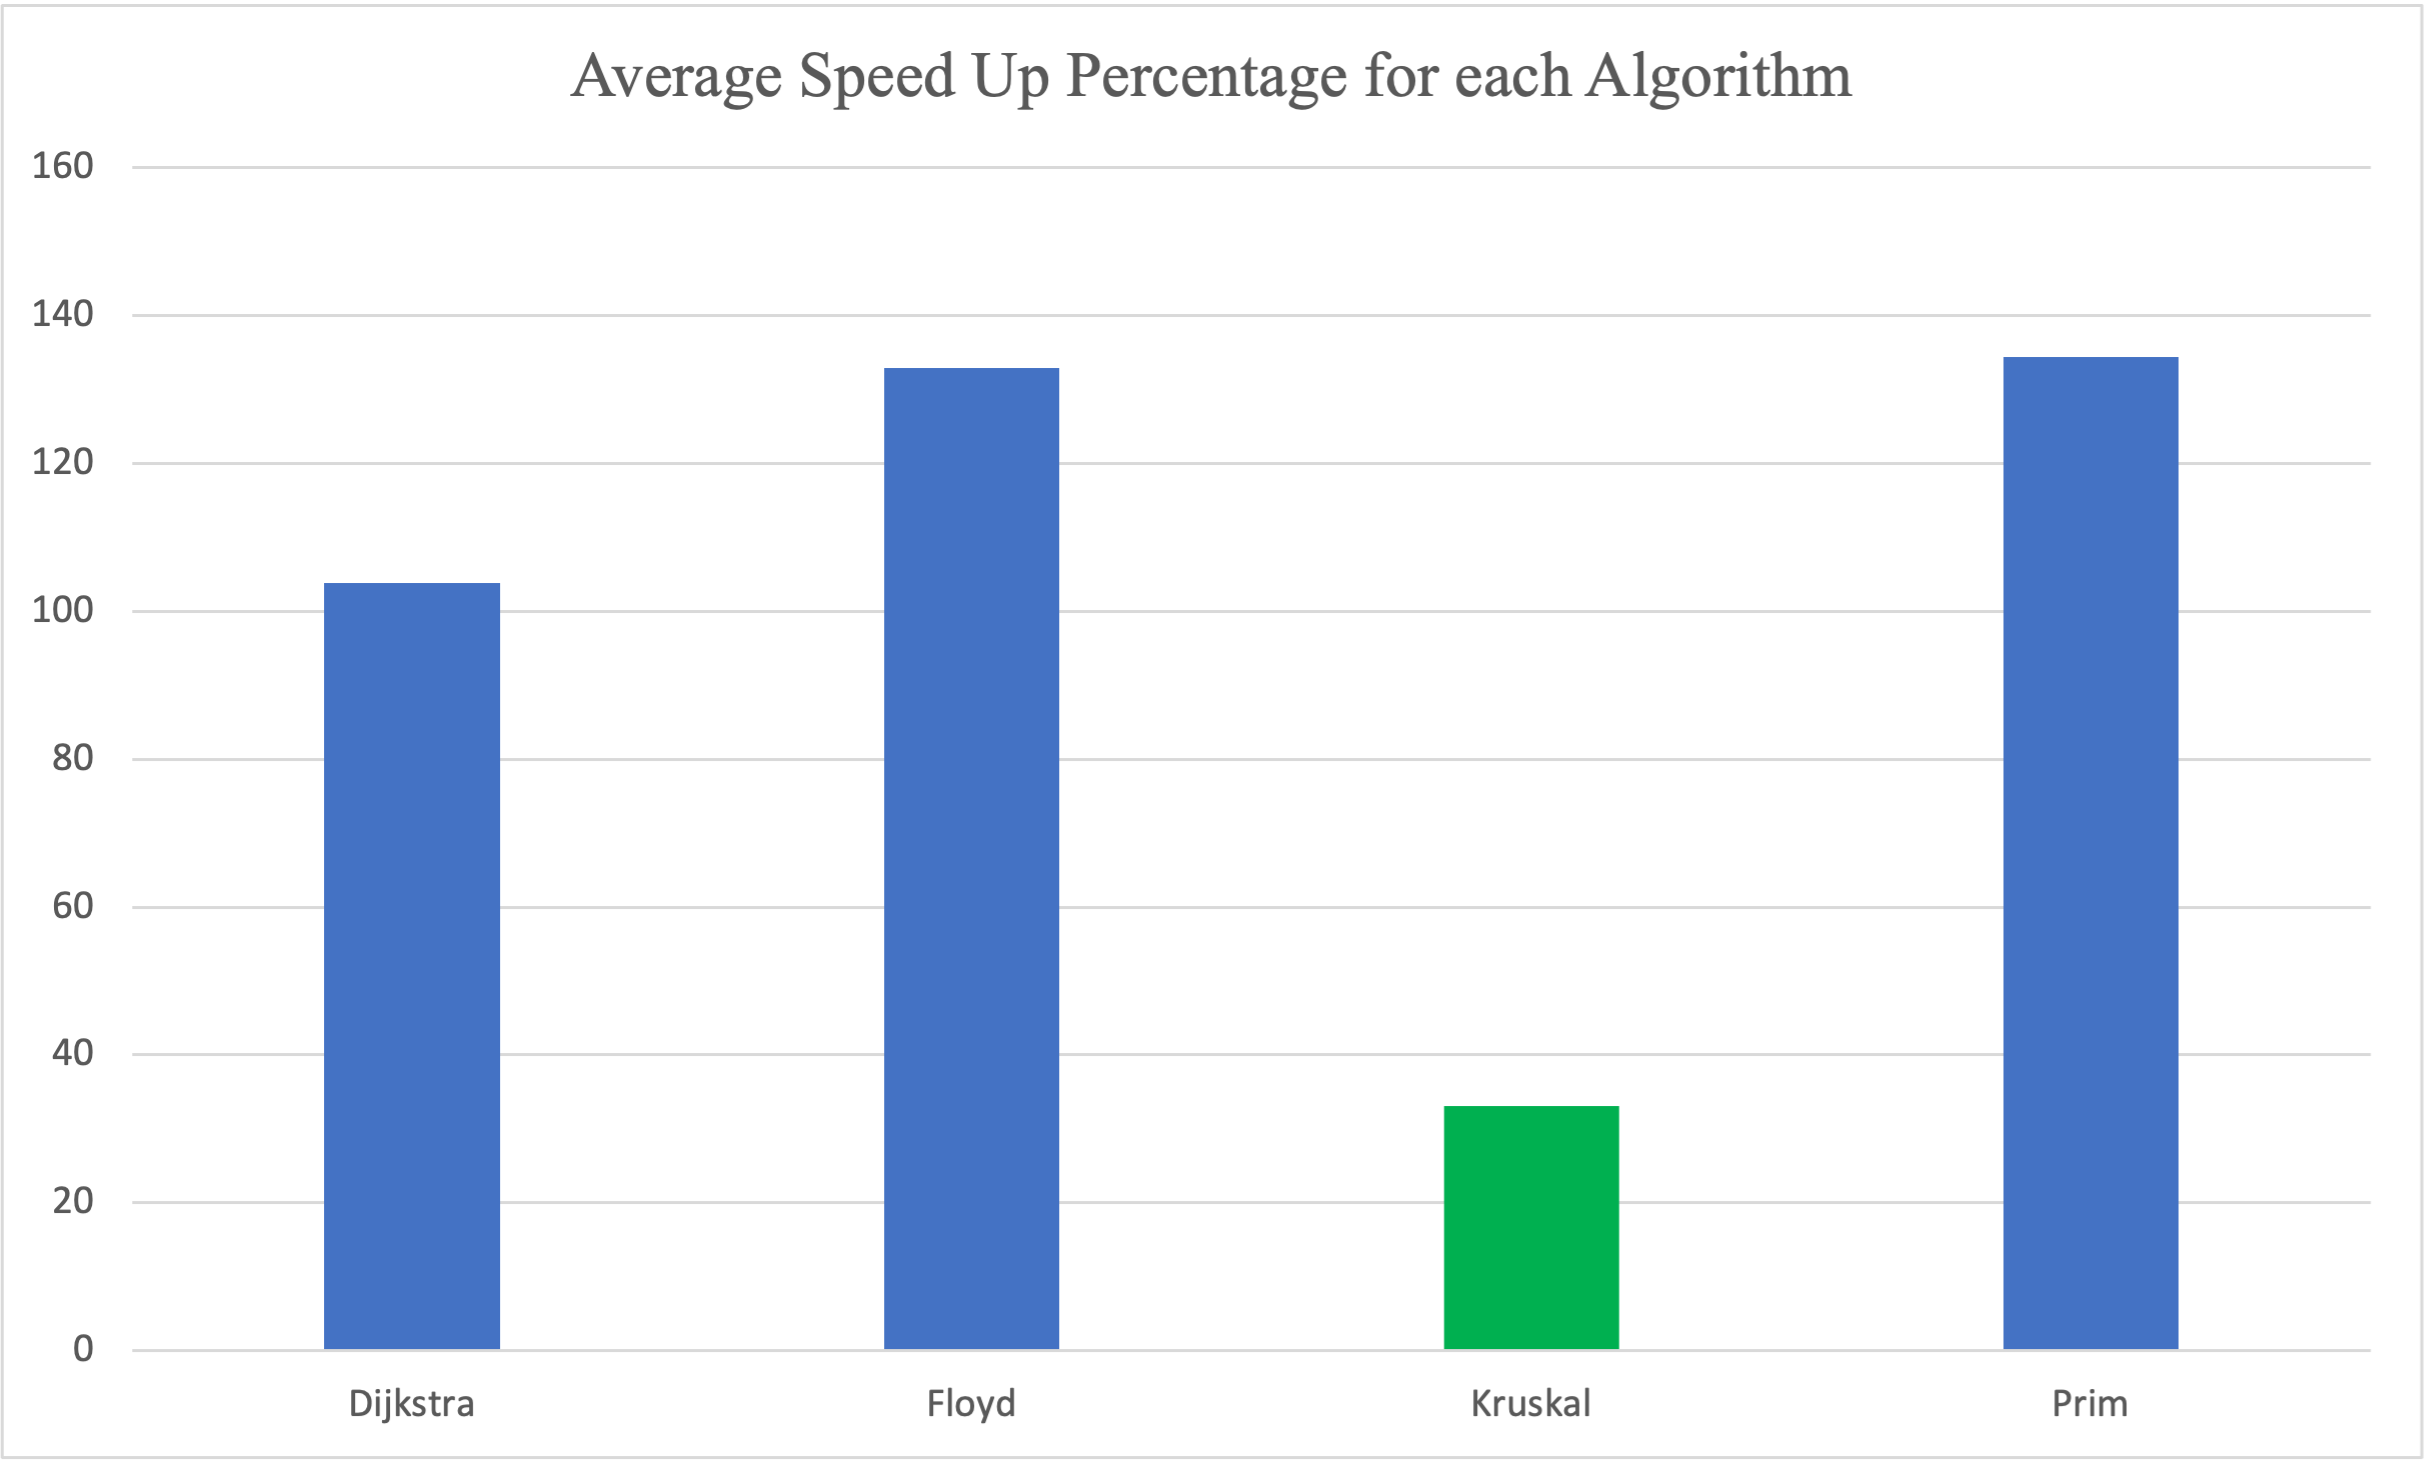
\includegraphics[scale=0.7]{avg-other-per}
\caption{\footnotesize{Average performance difference between Flask and Spin on each benchmarking algorithm, Kruskal is marked green}}
\captionsetup{aboveskip=0pt,font=it}
\end{figure}
\bigskip

We list out the data input size for the shortest path/MST algorithms to explore further. We found that the data input size for Kruskal's algorithm is a lot larger than other 3 other algorithms. The average data input size for Kruskal's algorithm is \textbf{1166666.67}, way larger than the algorithm with the second largest data input size, which is Dijkstra's algorithm with \textbf{4100}. In fact, \textbf{28355.285\%} larger!

\bigskip
\begin{table}[h!]
\centering
\begin{tabular}{||c c c c||} 
\hline
Name & Small & Medium & Large \\ [1ex] 
\hline\hline
 & & & \\
Dijkstra & 2500 & 4000 & 5800 \\ 
 & & & \\
Floyd-Warshall & 180 & 250 & 310 \\ 
 & & & \\
Kruskal & 400000 & 1000000 & 2100000 \\ 
 & & & \\
Prim & 400 & 550 & 680 \\ [1ex]
\hline
\end{tabular}
\caption{Data input sizes for shortest path/MST algorithms}
\label{table:time_complexity_1}
\end{table}
\bigskip

\newpage
\bigskip
\begin{figure}[hp]
\centering
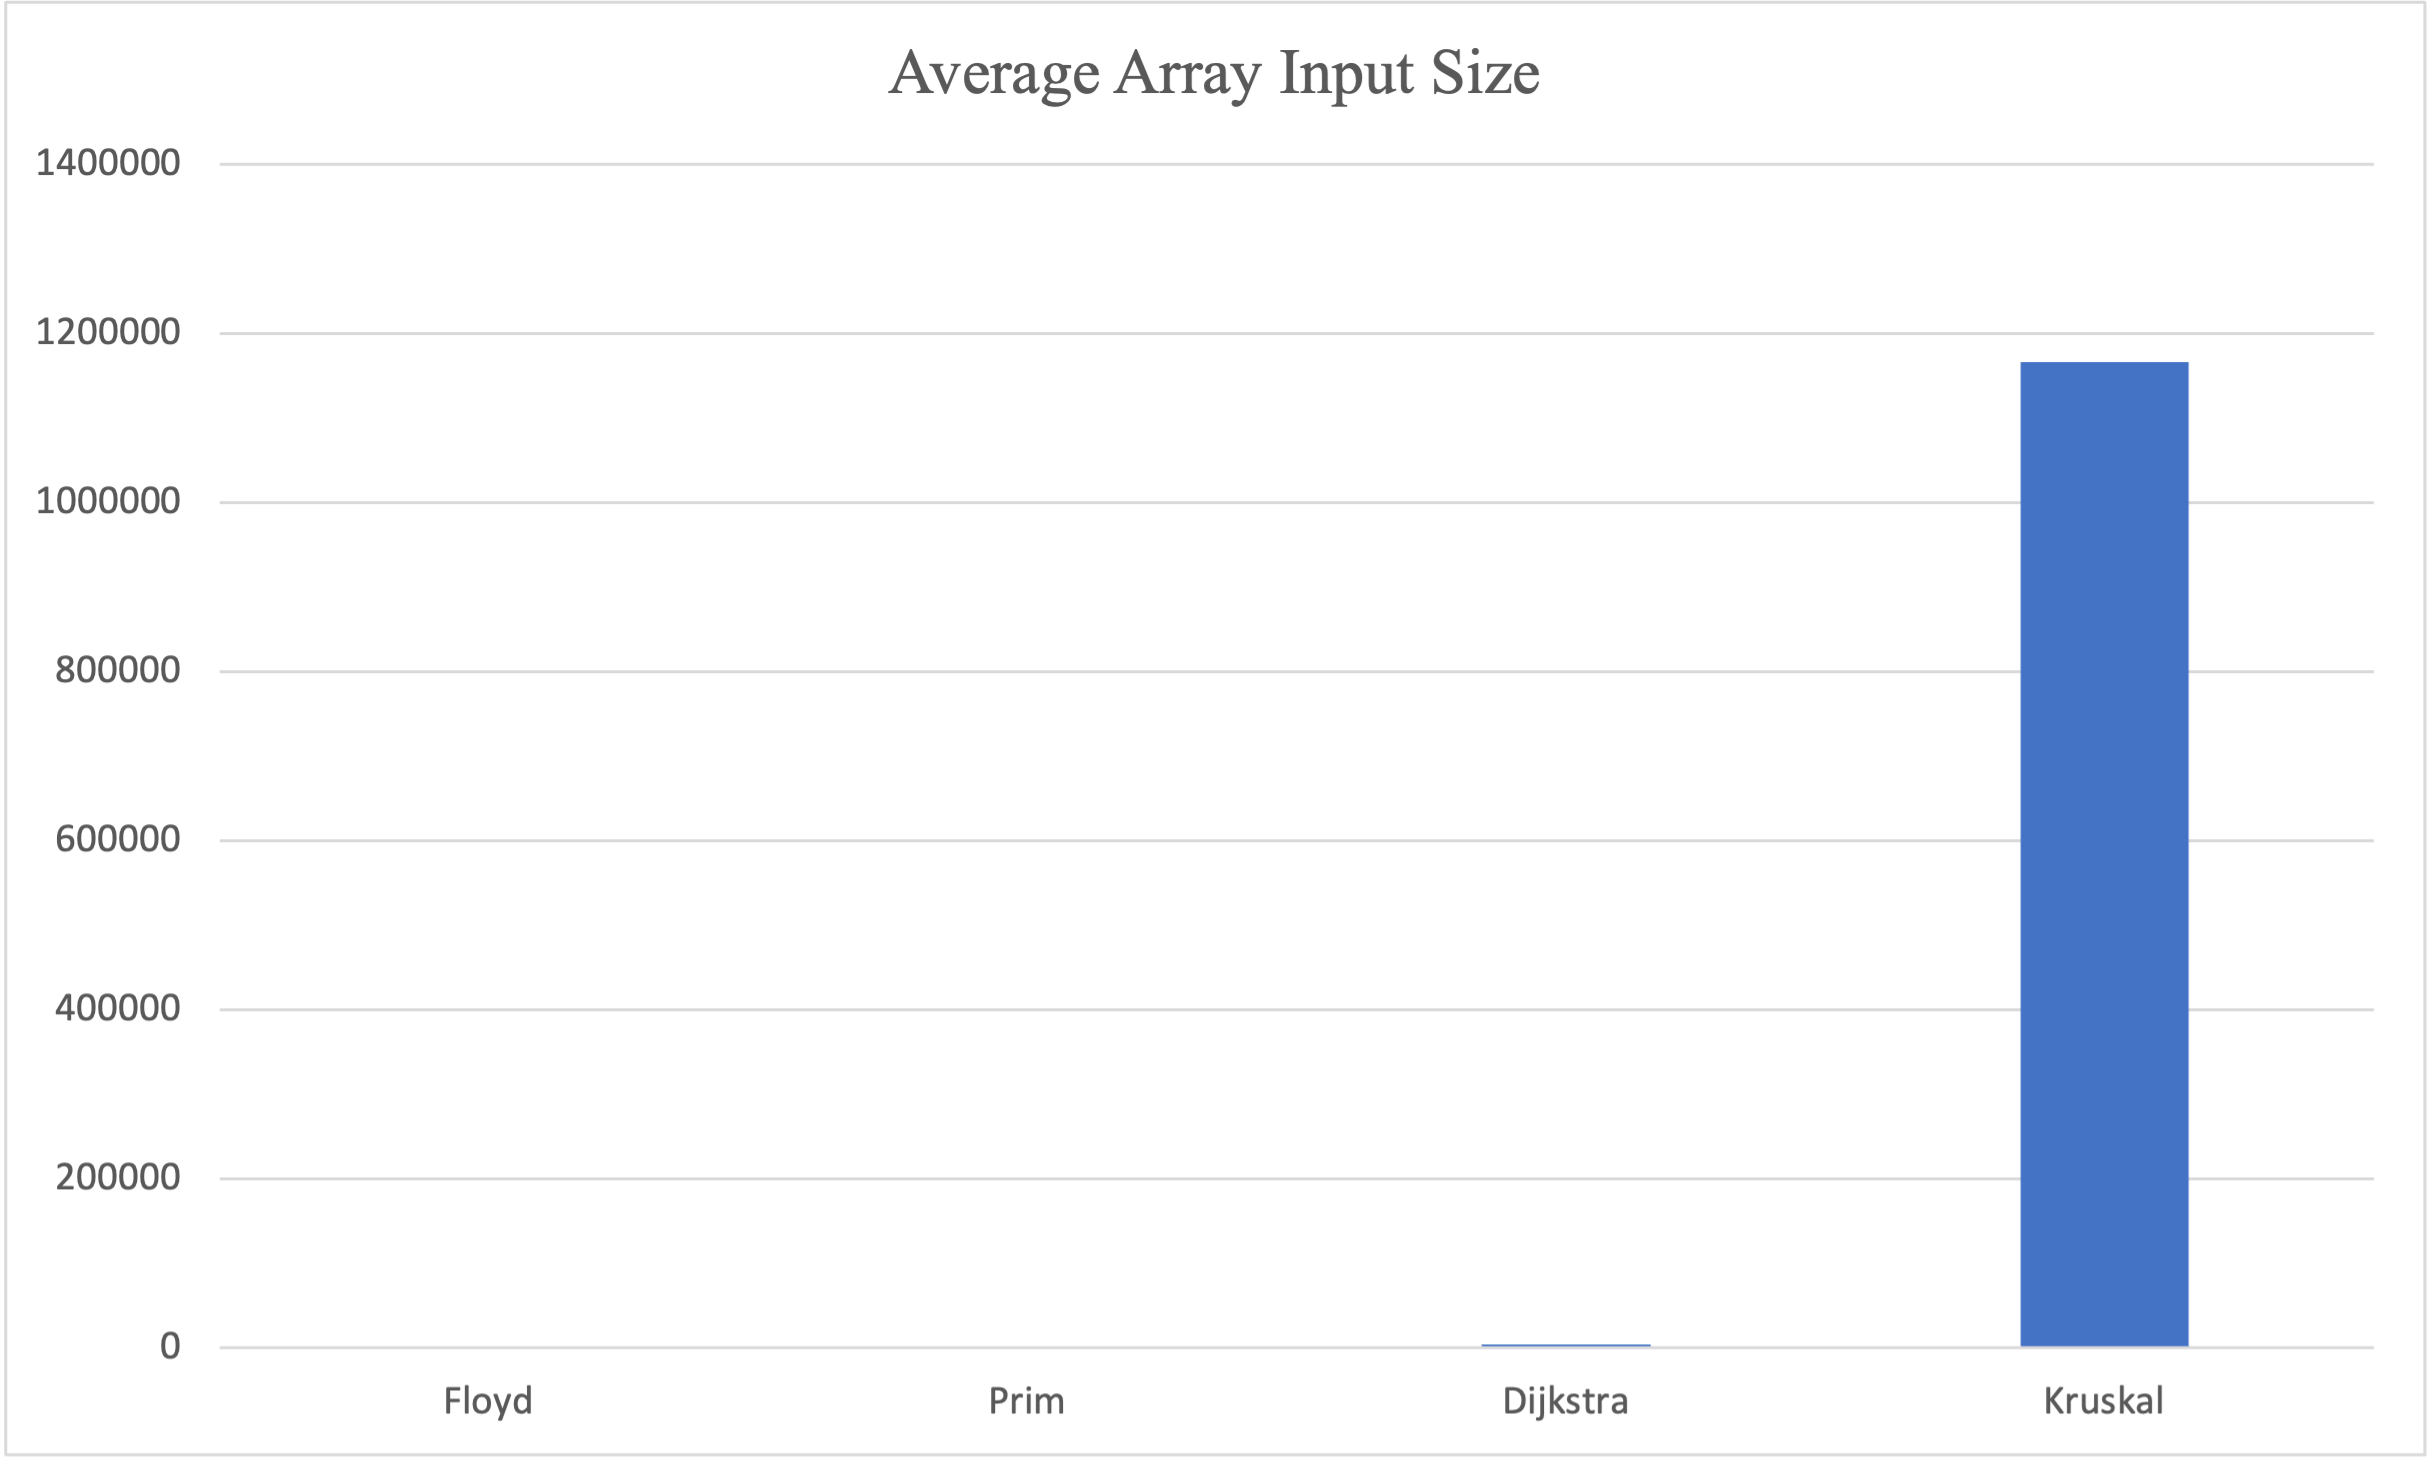
\includegraphics[scale=0.7]{avg-input-size-other}
\caption{\footnotesize{Average data input size for shortest path/MST algorithms (Sorted from small to large). Floyd and Prim's data input sizes are so small in contrast to Kruskal that we cannot see them at all in the graph}}
\captionsetup{aboveskip=0pt,font=it}
\end{figure}
\bigskip

From the table and the chart above, we recognise that there could be a correlation between the data input size with the average algorithm performance difference. This is a solid discovery as it is very much in alignment with the behaviour on the benchmarks for sorting algorithms' performance in the first stage of the experiment. In this case, the algorithm with the lowest performance difference \textbf{(Kruskal's algorithm)} also simultaneously has the largest data input size.

\subsection{Standard Deviation Analysis}

Just like in the first stage of the experiment, we ran each shortest path/MST algorithm \textbf{5} times to ensure the result data we get is consistent.

\bigskip
\begin{table}[h!]
\centering
\begin{tabular}{||c c c c||} 
\hline
Name & Standard Deviation ($\sigma$) & Confidence Interval & 95\% Confidence Interval \\ [1ex] 
\hline\hline
 & & & \\
Dijkstra (S) & 0.04 & 0.018 & 1.5632 ±0.0351 (±2.24\%) \\
 & & & \\
Dijkstra (M) & 0.044 & 0.02 & 4.1416 ±0.0385 (±0.93\%) \\
 & & & \\
Floyd (S) & 0.118 & 0.053 & 1.598 ±0.103 (±6.47\%) \\
 & & & \\
Floyd (M) & 0.109 & 0.049 & 3.8298 ±0.0955 (±2.49\%) \\
 & & & \\
Floyd (L) & 0.757 & 0.339 & 7.9802 ±0.664 (±8.32\%) \\
 & & & \\
Kruskal (S) & 0.167 & 0.075 & 1.853 ±0.146 (±7.88\%) \\
 & & & \\
Kruskal (M) & 0.28 & 0.125 & 4.9848 ±0.246 (±4.93\%) \\
 & & & \\
Prim (S) & 0.143 & 0.064 & 2.0054 ±0.125 (±6.23\%) \\
 & & & \\
Prim (M) & 0.089 & 0.04 & 4.9632 ±0.0782 (±1.58\%) \\
 & & & \\
Prim (L) & 0.147 & 0.066 & 9.3292 ±0.129 (±1.38\%) \\
 & & & \\
Dijkstra (S) & 0.137 & 0.061 & 3.119 ±0.12 (±3.86\%) \\
 & & & \\
Dijkstra (M) & 0.509 & 0.228 & 8.6162 ±0.446 (±5.18\%) \\
 & & & \\
Dijkstra (L) & 0.562 & 0.251 & 18.6322 ±0.492 (±2.64\%) \\
 & & & \\
Floyd (S) & 0.274 & 0.123 & 3.6254 ±0.24 (±6.63\%) \\
 & & & \\
Floyd (M) & 0.327 & 0.146 & 9.4122 ±0.286 (±3.04\%) \\
 & & & \\
Floyd (L) & 0.649 & 0.29 & 18.0462 ±0.569 (±3.15\%) \\
 & & & \\
Kruskal (S) & 0.232 & 0.104 & 2.5208 ±0.203 (±8.05\%) \\ [1ex]
\hline
\end{tabular}
\caption{Standard deviation for Flask framework}
\label{table:time_complexity_2}
\end{table}
\bigskip

\newpage
\bigskip
\begin{table}[h!]
\centering
\begin{tabular}{||c c c c||} 
\hline
Name & Standard Deviation ($\sigma$) & Confidence Interval & 95\% Confidence Interval \\ [1ex] 
\hline\hline
 & & & \\
Kruskal (M) & 0.439 & 0.196 & 6.4914 ±0.385 (±5.93\%) \\
 & & & \\
Kruskal (L) & 0.842 & 0.377 & 15.0142 ±0.738 (±4.92\%) \\
 & & & \\
Prim (S) & 0.22 & 0.098 & 4.2422 ±0.193 (±4.55\%) \\
 & & & \\
Prim (M) & 0.76 & 0.34 & 11.9216 ±0.666 (±5.58\%) \\
 & & & \\
Prim (L) & 1.049 & 0.469 & 23.4506 ±0.919 (±3.92\%) \\ [1ex]
\hline
\end{tabular}
\caption{Standard deviation for Flask framework (continued)}
\label{table:time_complexity_2}
\end{table}
\bigskip

In the above analysis for the standard deviation, similar to the discovery we made during the first stage of the experiment, we discovered that the larger the input data, the larger the standard deviation for the algorithm. For Flask, the average standard deviation for small input data size is \textbf{0.117} while the average standard deviation for large input data size is \textbf{0.452}, a \textbf{286.33\%} increase. This is even more visible when we look at the standard deviation for Spin benchmarks, the average standard deviation for small input data size is \textbf{0.216}, and the average standard deviation for large input data size is \textbf{0.776}. We are able to observe a similar increase in standard deviation at \textbf{286.33\%}.

\bigskip
\begin{figure}[hp]
\centering
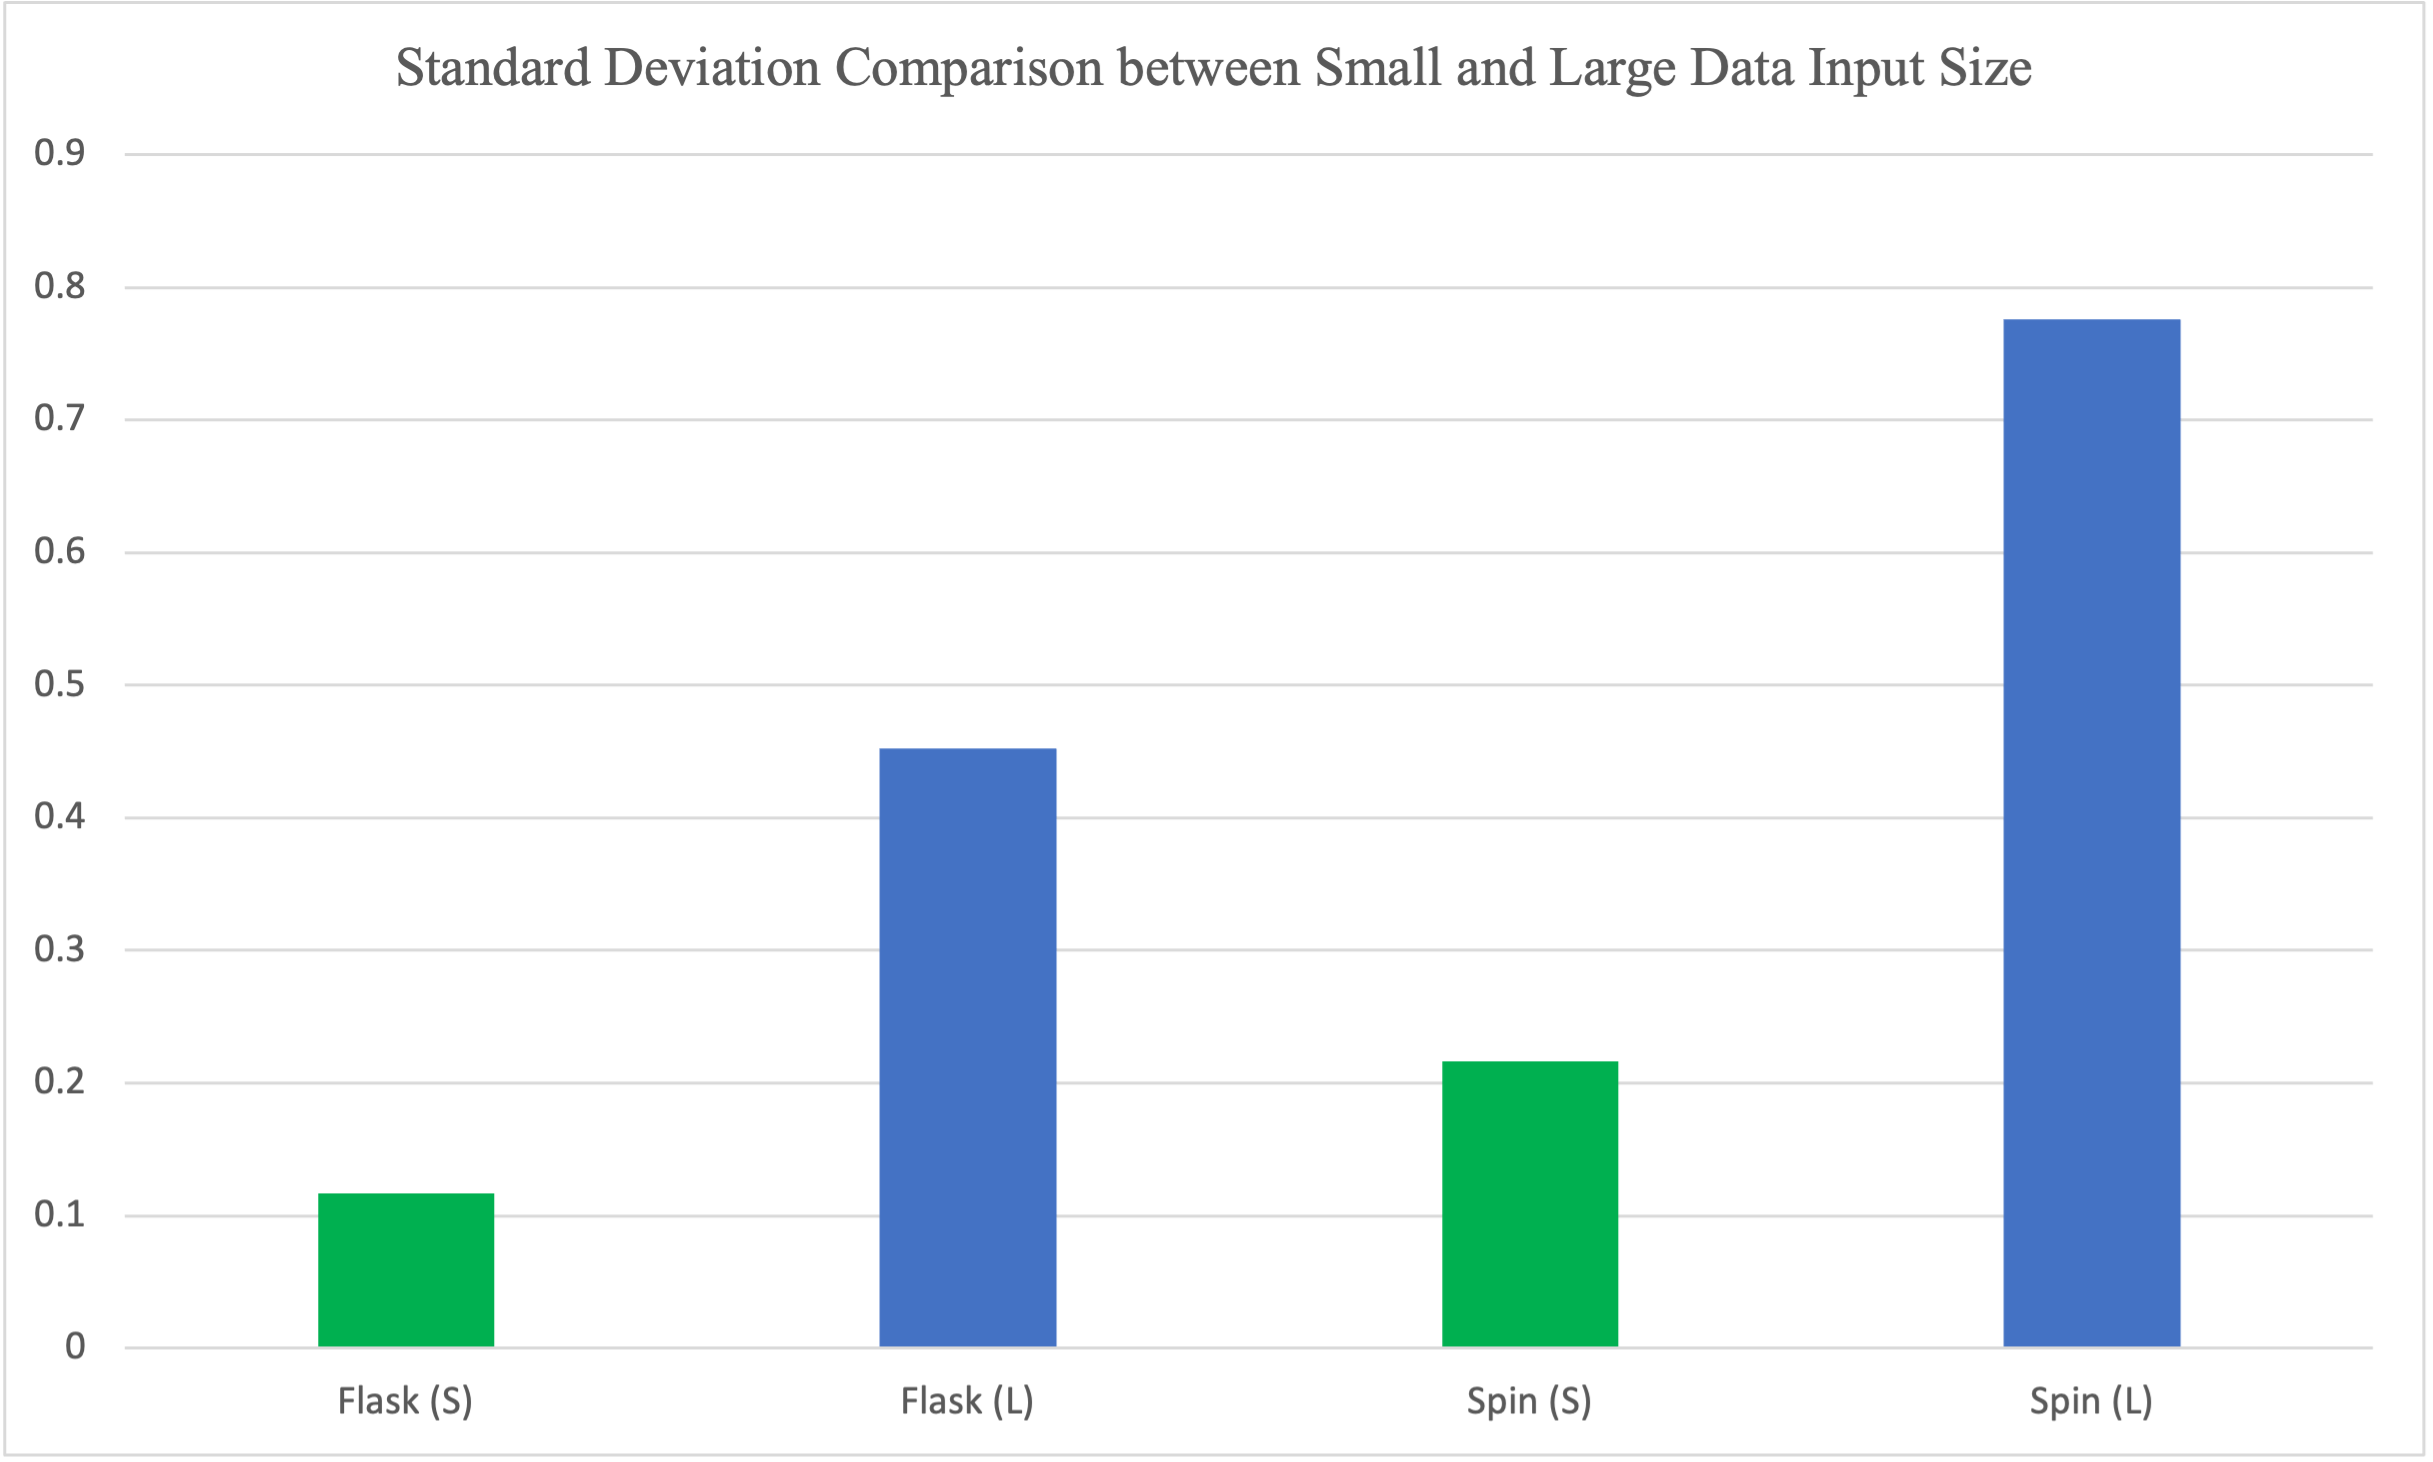
\includegraphics[scale=0.7]{sd-comp}
\caption{\footnotesize{Standard deviation comparison between small and large data input size on both Flask and Spin framework}}
\captionsetup{aboveskip=0pt,font=it}
\end{figure}
\bigskip